\documentclass[12pt,spanish,fleqn,openany,letterpaper,pagesize]{book}


\newpage

\NeedsTeXFormat{LaTeX2e}
\usepackage[lmargin=3cm, rmargin=3cm, top=2cm, bottom=2cm]{geometry}
\usepackage{amsfonts, amsmath, amsthm, latexsym, amssymb}
\usepackage{setspace}
\usepackage[spanish,es-tabla]{babel}
\usepackage{fancyhdr}
\usepackage{epsfig}
\usepackage{epic}
\usepackage{amscd}
\usepackage{here}
\usepackage{graphicx}
\graphicspath{ {images/} }
\usepackage{multirow}
\usepackage{multicol}
\usepackage{blindtext}
\usepackage{scrextend}
\usepackage{float}
\usepackage{subfigure}
\usepackage{titling}
\usepackage{titlesec}
\usepackage[usenames]{color}
\usepackage{hyperref}
\addtokomafont{labelinglabel}{\sffamily}
\spanishdecimal{.}
\hyphenation{que}
\renewcommand{\baselinestretch}{1.3}
\def\a{\alpha}
\def\b{\beta}
\def\e{\var
epsilon}
\def\t{\theta}
\def\g{\gamma}
\def\k{\kappa}
\def\ta{\tau}
\def\w{\omega}
\def\s{\sigma}
\def\d{\partial}

\def\N{\mathbb N}
\def\Z{\mathbb Z}
\def\Q{\mathbb Q}
\def\R{\mathbb R}
\def\C{\mathbb C}
\def\P{\mathbb P}
\def\E{\mathbb E}
\def\K{\mathbb K}
\def\S{\mathbb S}
\def\Rn{\mathbb R^n}
\def\En{\mathbb E^n}

\theoremstyle{definition}
\newtheorem{eje}{Ejemplo}
\newcommand\T{\rule{0pt}{2.6ex}} % Top strut
\newcommand\B{\rule[-1.2ex]{0pt}{0pt}}
\setlength{\parindent}{0pt}
\makeatletter
%\renewcommand{\fnum@figure}[1]{\textbf{\figurename~\thefigure}: \sffamily}
%\makeatother
\usepackage[labelfont={bf,sf}, tableposition=top]{caption}


%
\makeatletter
\let\ps@plain\ps@empty
\makeatother
%
\pagestyle{fancy}
\fancyfoot{}
\fancyhead{}
\fancyhead[L]{\scriptsize \leftmark}
\fancyhead[R]{\scriptsize \rightmark}
\fancyhead[R]{\thepage}
\renewcommand{\headrulewidth}{0.8pt}



\begin{document}
\frontmatter


\begin{titlepage}
\centering
\begin{center}
\includegraphics[scale=0.23]{USAlogo.jpg}
\end{center}
\vspace{2cm}
{\scshape\Huge Estudio de la correlación de contaminantes del aire de Bogotá. \par}
\vspace{2cm}
{\Large Autor: \par}
{\Large Michael Stiven Pinzón Rodríguez. \par}



\vspace{2cm}
{\itshape\Large Universidad Sergio Arboleda \par} 
Facultad de ciencias exactas e ingeniería\\
Maestría en Matemáticas Aplicadas
\vfill

\vfill
{\Large Bogotá D.C - 2022 \par}
 \end{titlepage}
\newpage


\begin{titlepage}
\centering
\begin{center}
\includegraphics[scale=0.23]{USAlogo.jpg}
\end{center}
\vspace{1cm}
{\scshape\Huge Estudio de la correlación de contaminantes del aire de Bogotá. \par}
\vspace{1cm}
{\Large Autor: \par}
{\Large Michael Stiven Pinzón Rodríguez. \par}

\vspace{1cm}
{\Large Tutora: \par}
{\Large Biviana Marcela Suárez Sierra. \par}
\vspace{1cm}
{\itshape\Large Tesis de grado presentada como requisito parcial para optar al título de: \par} 
{\itshape\Large \textbf{Magister en Matemáticas Aplicadas} \par} 
\vspace{1cm}
{\itshape\Large Universidad Sergio Arboleda \par} 
Facultad de ciencias exactas e ingeniería\\
Maestría en Matemáticas Aplicadas
\vfill

\vfill
{\Large Bogotá D.C - 2022 \par}
 \end{titlepage}


\newpage

\newpage



\chapter*{Agradecimientos}

En primer lugar, quiero agradecer a la Doctora Biviana Marcela Suárez Sierra, por su compromiso, paciencia y dedicación conmigo en la realización de este trabajo de grado, por haber confiado en mi y por compartirme sus ideas para poder llevar a cabo este trabajo. Por aceptar ser mi tutora aún sabiendo que no tenía conocimientos en programación y por haberme motivado a aprender al respecto para poderlo sacar adelante. 
También agradezco a la universidad Sergio Arboleda por permitirme la oportunidad de pertenecer a esta maestría y a los profesores, quienes aportaron innumerables cosas a mi profesión. 


\renewcommand{\contentsname}{Contenido}
\addcontentsline{toc}{chapter}{Introducción}
\addcontentsline{toc}{chapter}{Agradecimientos}
\tableofcontents
\listoffigures
\listoftables
\addcontentsline{toc}{chapter}{Bibliografía}
\mainmatter
\chapter*{Introducción}


La asociación o correspondencia entre dos variables, ha sido estudiada desde distintos puntos de vista y probada por diferentes autores. De acuerdo con Farlie (1960) en \cite{farlie} algunos de estos coeficientes de correlación son: 

\begin{enumerate}
\item Coeficiente de correlación de Pearson.
\item Coeficiente de correlación de Spearman.
\item Coeficiente de correlación de Kendall $\tau$
\item Probabilidad en concordancia. 
\end{enumerate}

Farlie (1960), afirma en \cite{farlie} que la eficiencia de cada uno de estos coeficientes no es muy conocida, sin embargo lo que si está dicho, es que ninguno en uniformemente mejor que el otro. De manera partícular el coeficiente de correlación es una herramienta útil, solo en algunos casos, de esta manera se utiliza la Cópula de Farlie-Gumbel-Morgenstern (FGM) para determinar para estimar el parámetro $\theta$ que representará la correlación entre dos parejas de contaminantes, estos son $PM_{10}$ vs $O_3$, $PM_{2.5}$ vs $O_3$ y $PM_{2.5}$ vs $PM_{10}$, para poder hacer esto, se seguirá el siguiente camino, en el capítulo número 1 se describirán algunos elementos de la inferencia bayesiana como el teorema de bayes, la creación de cadenas de Markov mediante el método de Monte Carlo (MCMC) y los algoritmos utilizados para lograr generar dichas cadenas. 

También se presentan algunos criterios de convergencia para los parámetros obtenidos mediante las simulaciones por el método MCMC, esto para determinar su validez y generar confianza en el módelo, estos criterios de convergencia son el de Geweke, que analiza dos partes de las cadenas construidas, el $10\%$ inicial y el $50\%$ final, verificando que la diferencia de sus medias sea mínima, cuando esto sucede, los parámetros son aceptados. De la misma manera se estudian otros criterios de convergencia como lo son el de Heidelberger-Welch, el de Raftery and Lewis y el de Gelman $\&$ Rubin. 
También se hace una descripción detallada del concepto de cópula junto con sus propiedades y conceptos previos necesarios para entenderlas y al finalizar este capítulo se describe la cópula utilizada para determinar la correlación de los tres pares de contaminantes. 

En el segundo capítulo se inicia el manejo de los datos analizados, para esto se inicia con una descripción de cada material contaminante junto con la reglamentación establecida por el ministerio de ambiente y desarrollo sostenible de Colombia. Esta descripción esta acompañada de los porcentajes en los cuales, durante el periodo comprendido entre el 2018 y el 2020, estos tres contaminantes analizados rebasan la norma establecida y se representa todo esto en tres series de tiempo diferentes construidas en el software R. Adicionalmente, se realiza el análisis de la gráfica de medias acumuladas que representa los datos de cada contaminante y se empieza a elaborar un modelo con el fin de encontrar los parámetros que se ajustan de la mejor forma a los datos conocidos. Se realizan tres modelos diferentes buscando un ajuste óptimo de los datos, el primero, \textbf{sin puntos de cambio}, no tiene en cuenta algúna afectación ocurrida durante los tres años, que muestre un cambio brusco en el comportamiento de los datos, en el segundo análisis, con \textbf{un punto de cambio}, se tiene en cuenta uno de los cambios mas representativos que hay en la serie de tiempo, para tomarlo como punto de cambio y hacer que el modelo cambie su comportamiento en ese punto dado. De igual manera en el tercer análisis \textbf{dos puntos de cambio}, se observa mejor el ajuste, dado que se configura el código programado para que asuma dos puntos específicos en los que hubo algún comportamiento drástico en los datos. 

El caítulo tres, corresponde al diagnóstico de convergencia para verficar si los resultados obtenidos en el capítulo dos, eran óptimos o debían ser modificados, para cada uno de los tres modelos se realizaron los tests hasta obtener resultados favorables que permitieran obtener unos parámetros adecuados, estos resultados dan paso al cuarto capítulo, donde se toman como referencia los parámetros obtenidos para el primer ajuste, \textbf{sin puntos de cambio} y se comienza el análisis bivariado. Buscando, mediante la cópula utilizada, el parámetro que determinará la correlación entre cada par de contaminantes, aquí se presentan los resultados numéricos obtenidos sobre esta correlación, encontrando cosas partículares sobre cada par de contaminantes. 

Finalmente, en el capítulo número cinco, se presentan algunas conclusiones de todo lo realizado en el desarrollo del presente trabajo de grado y se sugiere además la realización del modelo bivariado teniendo en cuenta los dos ajustes faltantes. 
\chapter{Preliminares}

\section{Inferencia bayesiana}
En el presente trabajo de grado, son necesarios algunos resultados importantes del curso Inferencia Bayesiana, es por eso que a continuación se presentan algunas definiciones y teoremas que son de gran utilidad para poder encontrar los diferentes parámetros que modelan los diferentes contaminantes y su respectiva correlación. 



%Se llama inferencia bayesiana a esa parte de la estadística que se encarga de utilizar la información conocida, los datos observados, la experiencia, la genética, etc., para poder hablar del futuro haciendo uso de la probabilidad. 
%Esto lo hace utilizando el teorema de bayes, el cual permite actualizar la probabilidad a medida que se obtienen nuevos datos. 

El análisis de datos Bayesiano es el nombre que se le da a cada uno de los métodos prácticos que se construyen para hacer inferencias a partir de datos conocidos, utilizando modelos de probabilidad \cite{infe_bayes}. Gracias a la experiencia o al conocimiento previo sobre algún tema particular, se pueden construir modelos que permiten realizar inferencias y tomar desiciones futuras, siempre enfocados en la mejora continua de los procesos. 

A este conocimiento previo se le denomina distribución a priori $P(\theta)$, cuya definición es una representación por medio de distribuciones de frecuencia que dependen de los datos ya conocidos. 

En el presente trabajo de grado, el interés está en encontrar conclusiones sobre la relación que tienen, dos a dos, tres contaminantes elegidos y de los cuales se tiene una información previa que en este caso será la experiencia necesaria para hacer uso de la teoria Bayesiana y enfocar el objetivo principal que será identificar la correlación entre dos procesos estocásticos. Esto se podrá hacer, siempre y cuando se establezca un modelo para cada uno de los tres contaminantes y también para los pares, para hacerlo, se utiliza la siguiente notación, $\theta$ denota cantidades de vectores no observables o parámetros poblacionales de interés y  $X$ los datos observados o conocidos con lo cuales se construirá el modelo, para este caso, el número de excedencias de los tres contaminantes durante los tres años analizados. 

En este sentido, la inferencia bayesiana se encargará de realizar conclusiones estadísticas sobre el parámetro $\theta$ a través de la probabilidad condicional, lo cual se escribe simplemente como $P(\theta | X$) \cite{infe_bayes}. En adelante, la expresión $p(\cdot|\cdot)$
denota una densidad de probabilidad condicional cuyos argumentos se podrán inferir del contexto  

\section{Teorema de Bayes}

En \cite{infe_bayes}, Gelman, A. et al, hacen una descripción un tanto sencilla para comprender lo que aporta a esta inverstigación, el teorema de Bayes, pues mencionan que para formular enunciados de probabilidad sobre $\theta$ dado $X$ se debe iniciar con un modelo que proporcione una distribución de probabilidad conjunta para $\theta$ y $X$. 
La función de densidad de probabilidad conjunta, como se menciona en \cite{infe_bayes} se puede escribir como el producto de dos densidades, la distribución a priori $P(\theta)$ y la distribución de muestreo $p(X|\theta)$ esto es: 
\begin{center}
\begin{equation}
p(\theta,X)=p(\theta)p(X|\theta)
\label{densidad}
\end{equation}
\end{center}

Aqui, aplicando la definición de probabilidad condicional a la ecuación \ref{densidad}, se obtiene lo siguiente:

\begin{center}
\begin{equation}
p(\theta|X)=\frac{p(\theta,X)}{p(X)}=\frac{p(\theta)p(X|\theta)}{p(X)}
\label{densidad_posterior}
\end{equation}
\end{center}

En la cual $p(X)=\sum_{\theta}p(\theta)p(X|\theta)$ para el caso discreto y $p(X)=\int p(\theta)p(X|\theta)d\theta $ en el caso continuo de $\theta$. 

Una forma equivalente a la ecuación \ref{densidad_posterior} no tiene en cuenta el factor $p(X)$, dado que este no depende de $\theta$ y con $X$ fijo, se puede considerar una constante, esto produce la \textit{densidad posterior no normalizada} \cite{infe_bayes}: 

\begin{equation}
p(\theta|y)\propto p(\theta)p(y|\theta)
\label{densidad_posterior_no_norm}
\end{equation}

Antes de que los datos $X$ sean considerados, la distribución de lo desconocido pero observado $X$, es: 

\begin{equation}
p(X)=\int p(X|\theta)d\theta=\int p(\theta)p(X|\theta)d\theta
\label{priori}
\end{equation}

La ecuación \ref{priori} es conocida como la \textit{distribución marginal de $X$} sin embargo un nombre que la describe mejor es \textit{distribución predictiva a priori}, priori, porque no esta condicionada a una observación previa del proceso y predictiva porque es la distribución para una cantidad que es observable. 

Ya una vez se tienen los datos $X$ observados, se pueden predecir datos observables desconocidos, $ \widetilde{X}$, la distribución de estos datos es llamada \textit{distribución predictiva posterior}, posterior porque esta condicionada a los $X$ observados y predictiva porque es una predicción para los $ \widetilde{X}$ observables. 

\begin{equation} \label{posterior}
\begin{split}
p(\widetilde{X}|X) & = \int p(\widetilde{X},\theta|X)d\theta \\
 & = \int p(\widetilde{X}|\theta,X)p(\theta|X)d\theta\\
 & = \int p(\widetilde{X}|\theta)p(\theta|X)d\theta
\end{split}
\end{equation}

Cuando se observa $X_1, X_2, \dots X_n$, estos datos ya no representan una variable aleatoria, de esta manera la distribución $p(x|\theta)$ se convierte en una función solo de $\theta$. A esta función se le conoce como \textit{verosimilitud} y se denota al igual que en \cite{tesisbiviana} como $L(D|\theta)$.

Dado que el presente trabajo de grado es una consecuencia de la tesis de doctorado de Suarez, B. (2020) \cite{tesisbiviana}, la notación referente a los datos observados es la misma, por la tanto aquí también, si $N$ es el número total de excedencias de alguno de los tres contaminantes estudiados, localizados en los días $D={d1, d2, \dots , d_N}$ y $\theta$ el parámetro desconocido del modelo, entonces de la formula de Bayes se tiene qué: 

\begin{equation}
\label{verosimilitud}
p(\theta|D)=\frac{p(D|\theta)p(\theta)}{p(D)}\propto L(D|\theta)p(\theta)=\prod_{i=1}^N p(d_i|\theta)p(\theta)
\end{equation} 


\section{Método Monte Carlo vía Cadenas de Markov (MCMC)[Jiménez (2015)]} 

Los métodos MCMC, cuyas siglas provienen de su nombre en inglés: \textit{Markov Chain Monte Carlo}, son algoritmos que simulan el comportamiento de variables aleatorias para poder estimar parámetros desconocidos de las funciones de probabilidad de dichas variables. En el presente trabajo de grado se realizará la inferencia sobre la función aposteriori, $p(\theta|X)$

En \cite{MCMC} se presentan los siguientes dos pasos sobre la aplicación de las técnicas MCMC: 

\begin{enumerate}
\item Generar una muestra $X_1, \dots, X_n$ mediante una cadena de Markov cuya distribución estacionaria sea la buscada. 
\item Tomar medias muestrales (integración Monte Carlo) y realizar inferencias sobre la muestra. Para construir estas cadenas de Markov, existen dos familias de algoritmos que son: El algoritmo de Metropolis-Hastings y el muestreo de Gibbs, los cuales serán descritos a continuación. 
\end{enumerate}
\subsection{Algoritmo de Metropolis Hastings}

Suárez, B. (2020), en \cite{tesisbiviana} cita a Metropolis (1949), Hastings (1970) de la siguiente manera: 

Sea $f(\cdot)$ una distribución de la cual se quiere generar valores, pero que no es posible hacerlo directamente. El algoritmo Metropolis-Hastings dice que apartir de una distribución condicional $q(y|x)$, de la que se puede generar valores facilmente, se crea una secuencia de observaciones $X_1$, $X_2$, $\dots,$ cuya distribución estacionaria es $f(\cdot)$. El algoritmo es: 

Sea $X_0=x_0$ el valor inicial, generado a partir de una distribución inicial adecuada. Para $n=0,1,2,\dots,$ si el estado actual es $X_n=x$, se obtiene $X_{n+1}$ así: 

\begin{enumerate}
\item Se genera un valor candidato $y$ usando $q(\cdot | X_n=x)$
\item Se evalúa $\a(x,y)=min \left[ \frac{f(y)q(x/y)}{f(x)q(y/x)},1\right]$

\item Asigne el valor a $X_{n+1}$ de la siguiente manera: 

\begin{displaymath}
X_{n+1} = \left\{ \begin{array}{l}
y \text{ con probabilidad } \a(x,y) \\
x \text{ con probabilidad } 1-\a(x,y) 
\end{array}
\right.
\end{displaymath}
\end{enumerate}

Aquí, para ejecutar el paso 3, se genera $U$ usando una distribución $uniforme(0,1)$ si $U<\a, X_{n+1}=y;$ en otro caso $X_{n+1}=x$


\subsection{Muestrador de Gibbs}

Sea $X=X_1, X_2, \dots ,X_{k-1}$ un vector aleatorio. El muestreador de Gibbs, arroja un resumen inferencia de la distribución conjunta $p(X)=p(X_1,X_2,\dots,X_k)$. Suponga que sea relativamente fácil generar valores de las funciones de densidad condicional completas denotadas por $p(X_1|X_2, \dots , X_k), p(X_i|X_1,\dots,X_{i-1},X_{i+1}), \dots ,X_k),$ para $i=2,\dots,k-1$ y $p(X_k|X_1,\dots,X_{k-1})$.

Dado un bector inicial $X^{(0)}=(X_1^{(0)},X_2^{(0)}),\dots,X_k^{(0)}$ obtenido de acuerdo a alguna distribución adecuadad, se implementa el siguiente proceso iterativo. 

Para $n=1,2,\dots,$ sea $X^{(n-1)}=(X_1^{(n-1)},\dots,X_k^{(n-1)})$, entonces 

\begin{enumerate}
\item Genere $X_1^{(n)}$ usando $P(\cdot|X_2^{n-1},\dots,X_k^{n-1})$

\item Para $i=2,3,\dots,k-1,$ genere $X_i^n$ usando $P(\cdot |X_1^{(n)},\dots,X_{i-1}^{(n)},X_{i+1}^{(n)},\dots,X_{k}^{(n-1)})$

\item genere $X_k^{(n)}$ usando $P(\cdot | X_1^{(n)},\dots,X_{k-1}^{(n)})$,

\item Haga $X^{(n)}=(X_1^{(n)},\dots,X_k^{(n)})$ y regrese al ítem 1, con $n$ en el lugar de $n-1$ y $n+1$ en lugar de $n$.

La sucesión $X^{(1)},X^{(2)},...,$ con $X^{(i)}=(X_1^{(i)},X_2^{(i)},\dots,X_k^{(i)}), \text{  } i=1,2,\dots$ es una realización de una cadena de Markov cuya distribución de transición está dada por: 


\begin{equation} \label{gibbs}
\begin{split}
P(X^{(t+1)}|X^{(t)}) & = p(X_1^{(t+1)}|X_2^{(t)},\dots,X_k^{(t)} ) \\
 & \times \prod_{i=2}^{k-1}p(X_i^{(t+1)}|X_1^{(t+1)},\dots,X_{i-1}^{(t+1)},X_{i+1}^{(t)},\dots,X_{k-1}^{(t)}) 
 \\
 & \times p(X_{k}^{(t+1)}|X_{1}^{(t+1)},\dots,X_{k-1}^{(t+1)}),
\end{split}
\end{equation}


Lo cual bajo condiciones adecuadas converge a $f(\cdot)$ cuando $n$ tiende a infinito. 
\end{enumerate}

\section{Algunos diagnósticos de convergencia para los parámetros estimados}




Como ya se mencionó, para la elaboración del presente trabajo de grado, se generan cadenas de Markov para estimar los parámetros deseados. En esta sección se presentan algunos criterios que permiten generar confianza en los modelos, pues se evalua mediante su convergencia si son fiables o no. A continuación se presentan algunas de estas pruebas de convergencia:

 

\subsection{Método Geweke [Geweke (1992)]}

Geweke, J. (1992), \cite{geweke} citado por Suárez, B. (2020) \cite{tesisbiviana}  brinda un diagnóstico de convergencia en el cual establece que si el comportamiento del $10\%$ inicial de la cadena de Markov inicial es igual al $50\%$ final, entonces el estadístico de Geweke tiene una distribución normal estándar asintótica, es decir, $Z_n$, es tal que cuando $n\rightarrow \infty$ su distribución es una normal con parámetros $(0,1)$, aquí:


\begin{equation}
\label{estadistico}
Z_n=\frac{\sqrt{T}(\mu_A-\mu_B)}{\sqrt{\frac{\s_A^2}{r_A}+\frac{\s_B^2}{r_B}}}
\end{equation}

Con $T$ el número de iteraciones, $\mu_A$, $\mu_B$ medias y $\s_A^2$, $\s_B^2$ varianzas del primer y último segmento respectivamente, además $T_A=r_AT$ y  $T_B=r_BT$ con $r_A$ y $R_B$ proporciones de la longitud de la cadena del primer y último segmento. 


\subsection{Método Heidelberger-Welch}

Este modelo calcula un test estadístico para aceptar o rechazar la hipotesis nula de que la cadena de Markov corresponde a una distribución estacionaria. El método consiste de dos partes, en la primera se establece una cadena de $N$ iteraciones y se analiza, mediante el estadístico de prueba, si la cadena es estacionaria o no, cuando la hipotesis nula es rechazada, se descarta el $10\%$ inicial de la cadena y se repite el proceso, esto se hace hasta que la hipotesis nula es aceptada o hasta llegar al $50\%$ de la cadena. Si no se puede aceptar la hipotesis nula se dice que la cadena falla y que se debe elegir un mayor número de iteraciones. 

En la segunda parte del test, cuando la cadena o una parte de ella pasó la primera parte, se calcula el error estándar de la media y se calcula un intervalo de confianza para la media. 

Si la mitad del ancho de este intervalo de confianza construido es menor que un $\epsilon$ se puede decir que el tamaño de la nueva cadena es suficiente para estimar la media con precisión. \cite{romo}

\subsection{Método Gelman and Rubin}

En 1992, Gelman and Rubin plantearon una prueba de convergencia para determinar la veracidad de los parámetros estimados mediante cadenas de Markov. Este criterio de convergencia, consiste analizar $n$ cadenas independientes, 
y esta basado en estimar las varianzas $\s ^2 $ de $\theta$ por medio de un estimador $V$, el cual es construido promediando los estimadores obtenidos en cada cadena de Markov. Matemáticamente hablando, El Adlouni et al. (2006), citando a Gelman and Rubin (2006), presentan en \cite{adlouni} una descripción del algoritmo: 

Denotan, en primer lugar, $\theta_i^t=\theta(x_i^t)$ como la funcional evaluada en le $t-esima$ observación de la cadena $i$,

\begin{equation}
\overline{\theta}_i^{.}=\frac{1}{n}\sum_{t=n+1}^{2n} \theta_i^t , \overline{\theta}_{.}^{.}=\frac{1}{m} \sum_{i=1}^m \overline{\theta}_i^{.}, s_i^2=\frac{1}{n-1} \sum_{t=n+1}^{2n}(\theta_i^t-\overline{\theta}_i^{.})^2
\end{equation}

A partir de lo anterior, en \cite{adlouni} definen el estimador de ka siguiente manera: 

\begin{equation}
V=\frac{n-1}{W}+\left(1+\frac{1}{m}\right)\frac{B}{n}
\end{equation}

Donde $\frac{B}{n}$ representa las medias de la secuencia $m$ y es de la siguiente forma: 
\begin{equation}
\frac{B}{n}=\frac{1}{m-1}\sum_{i=1}^m(\theta_i^{.}-\overline{\theta}_{.}^{.})^2,
\end{equation}

$W$, es la media de las $m$ varianzas de la secuencia, $s_i^2$ y esta dada por: 

\begin{equation}
W=\frac{1}{m}\sum_{i=1}^m s_i^2
\end{equation} 

Con la información anterior, es posible construir un estimador $R_c$, el cual según Gelman and Rubin (1998), citados en \cite{adlouni}, si tiene valores muy grandes, hay dos posibilidades. 

\begin{enumerate}
\item La varianza $V$ se puede disminuir para mas simulaciones. 

\item $W$ puede disminuir para mas simulaciones. 
\end{enumerate}

En cambio, si el estimador de Gelman y Rubin, se encuentra cerca de 1, se puede concluir que cada una de los $m$ conjuntos de n sumulaciones observadas esta cerca de la simulación objetivo. 


\subsection{Método Raftery and Lewis} 

Raftery and Lewis (1992), proponen un método apropiado para determinar el número de iteraciones necesarias para calcular un quantil de la cadena de markov construida. Además analizan la longitud de ejecuación para que la probabilidad resultante se encuentre en un intervalo $[q-\epsilon,q+\epsilon]$,  esta presición requerida $\epsilon$ se encuentra con una probabilidad $(1-\alpha$  \cite{Roy}

En el software R, por medio de la función \textit{Raftery.Diagnostic} se obtienen los resultados de este criterio de convergencia, uno de estos resultados es la matriz \textit{resmatrix} en la cual se observan los resultados: burn-in sugerido,un número $N$ que es el número de iteraciones realizadas, un $N_min$ que es el número minimo de iteraciones sugeridas y un factor de dependencia $I$ el cual es determinado de la siguiente manera: $I=\frac{N}{N_{min}}$, el cual tiene la siguiente interpretación: $I>5$ indica que  hay relación de dependencia entre cada uno de los estados de la cadena, sugiriendo entonces que se deben modificar algunos de los valores propuestos en el modelo. \cite{tesisbiviana}, \cite{Rdoc}
\section{Funciones cópula}

El interés en el presente trabajo está, en determinar la correlación de dos procesos estocásticos relacionados con la contaminación del aire de la ciudad de Bogotá, para eso se hará uso de las funciones cópula, las cuales, dos a dos, darán un valor $\theta$ que determinará si la correlación es negativa, positiva o cero, arrojando resultados en el intervalo $[-1,1]$ 


\section{Definición de función Cópula[Nelsen (2006) \cite{nelsen}]}

Las cópulas son funciones que determinan distribuciones multivariadas a partir de las distribuciones marginales de una dimensión.

\textbf{Preliminares:}
Durante el proyecto se trabajará con la siguiente notación: 
\\
Se define $\R$ como la recta real usual, y $\overline{\R}$ como la recta real $[-\infty,\infty]$, en este caso $\overline{\R}^2$ denota el plano real extendido $\overline{\R}\times\overline{\R}$. Un rectángulo en $\overline{\R}^2$ es el producto cartesiano $B$ de dos intervalos cerrados: $$B=[x_1,y_1]\times[x_2,y_2]$$  Se define también el cuadrado unitario $\textbf{I}^2$ como el producto $\textbf{I}\times \textbf{I}$, donde $\textbf{I}=[0,1]$.

\vspace{0.5cm}
\textbf{Definición 1:} Una función real $2-place$ $H$ se define como una función cuyo dominio $DomH$ es un subconjunto de $\overline{\R}^2$ y cuyo rango, $RanH$ es un subconjunto de $\R$. 
\vspace{0.5cm}

\textbf{Definición 2:} Sea $S_1$ y $S_2$ subconjuntos no vacíos de $\overline{\R}$, y sea $H$ una función real $"2-place"$ tal que su dominio es $S_1 \times S_2$. Sea $B=[x_1,y_1]\times[x_2,y_2]$ un rectángulo cuyos vértices están estan en el $DomH$. Entonces el $H-volume$ de $B$ está dado por: 

$$V_H(B)= H(x_2,y_2)-H(x_2,y_1)-H(x_1,y_2) +H(x_1,y_1)$$

\vspace{0.4cm}
\textbf{Definición 3:} Una función real $2-place$ es $2-creciente$ si $V_H(B)\geq 0$ para todos los rectángulos $B$ cuyos vértices están en el dominio de $H$. 


Dada la información anterior, es posible ahora definir lo que son las Cópulas, pues son un concepto fundamental en el desarrollo del presente trabajo. Sin embargo para definirlas, antes es necesario definir lo que es una subcópula: 


\textbf{Definición 4:} Una subcópula $2-dimensional$ es una función $C$ con las siguientes propiedades:

\begin{enumerate}
    \item $DomC'=S_1 \times S_2$, donde $S_1$ y $S_2$ son subconjuntos de $\textbf{I}$ que contienen a $0$ y a $1$;
    \item $C'$ es cerrado y $2-creciente$
    
    \item Para cada $u$ en $S_1$ y cada $v$ en $S_2$,
    
    $$C'(u,1)=u \text{ y } C'(1,v)=v$$
\end{enumerate}

\textbf{Definición 5:} Una cópula $2-dimensional$ es una \textit{2-subcopula C} cuyo dominio es \textbf{${I}^2$}. 

De forma equivalente, una cópula es una función $C$ de $\textbf{I}^2$ en $\textbf{I}$ que satisface las siguientes propiedades. 

\begin{enumerate}
    \item Para cada $u, v$ en $\textbf{I}$, 
    $$C(u,0)=0=C(0,v) $$
    y
    $$C(u,1)=u \text{ y } C(1,v)=v; $$ 
    
    \item Para cada $u_1, u_2, v_1, v_2 $ en $\textbf{I}$ tal que $u_1 \leq u_2$ y $v_1 \leq v_2$,
    
    $$C(u_2,v_2)-C(u_2,v_1)-C(u_1,v_2)+C(u_1,u_2)\geq 0  $$
    
\end{enumerate}


\textbf{Teorema 2.1} (Teorema de Sklar \cite{sklar}).
\textit{Sea $F(\cdot,\cdot)$ una distribución conjunta con distribuciones marginales $F_1(\cdot)$ y $F_2(\cdot)$ respectivamente. Entonces, existe una cópula $C(\cdot,\cdot)$ tal que: }


\begin{equation}
F(x,y)=C(F_1(x),F_2(y)),\text{ para todo }x,y \in (-\infty,\infty)
\label{teosklar}
\end{equation}

La demostración de este teorema se puede encontrar en \cite{sklar}. 

En \cite{tesisbiviana}, Suarez (2020), hace uso de las funciones cópulas para determinar de manera detallada la función de riesgo bivariada $\lambda(t_1,t_2)$, la función de media acumulada (apróximada) $M(t_1,t_2)$ y la función de riesgo acumulada bivariada $m(t_1,t_2)$. 


\section{Cópula Farlie-Gumbel-Morgenstern (FGM)}

Existen diferentes cópulas propuestas, dependiendo de la situación en cuestión, para este estudio, al igual que en \cite{tesisbiviana} se utilizará la copula propuesta por Morgenstern (1956), citado por Fraile(1960) en \cite{farlie} cuyas marginales son Weibull. 

\textbf{Distribución bivariada Weibull:}


\begin{equation}
\label{copulafarlie}
F(x)G(x)[1+\theta\{1-F(x)\}\{1-G(x)\}]
\end{equation}

En la cual, $F(x), G(x) \in [0,1]$ y $\theta\in [-1,1]$

Suárez. B, (2020) en \cite{tesisbiviana} en el capítulo $3.2$ realiza una descripción detallada de la manera como se obtienen las funciones mencionadas anteriormente. Esto lo hace inicialmente, partiendo de que las funciones $F(x)=F_1(t_1), G(x)=F_2(t_2)$ sean las funciones marginales definidas de la siguiente manera: 

\begin{equation}
\label{marginales}
F_i(t_i)=1-\exp\left\lbrace-\left(\frac{t_i}{\s_i}\right)^{\a_i}\right\rbrace, \text{ con } \a_i, \s_i >0, i=1,2.
\end{equation}

De esta manera, al sustituir las marginales \ref{marginales} en la ecuación \ref{copulafarlie}, se obtiene: 

\begin{equation}
\label{funcionF}
\begin{split}
F(t_1,t_2) & = \left(1-\exp\left\lbrace-\left(\frac{t_1}{\s_1}\right)^{\a_1}\right\rbrace\right)\left(1-\exp\left\lbrace-\left(\frac{t_2}{\s_2}\right)^{\a_2}\right\rbrace\right)\\
 & \times \left(1+\theta\exp\left\lbrace-\left(\frac{t_1}{\s_1}\right)^{\a_1}-\left(\frac{t_2}{\s_2}\right)^{\a_2}\right\rbrace\right)
\end{split}
\end{equation}


\textbf{Función de densidad conjunta Weibull:}
\begin{equation}
\label{densidad_conjunta}
f(t_1,t_2)=f_1(t_1)f_2(t_2)[1+\theta[1-2F_1(t_1)][1-2F_2(t_2)]]\end{equation}

Donde $f_i(\cdot)$ es la función de densidad asociada a $F_i(\cdot), i=1,2.$


\textbf{Función de riesgo acumulada:}

La ecuación \ref{riesgo_acumulada} es una de las más importantes en el presente documento, pues es la cópula que determina el modelo de programación utilizado para determinar los parámetros de correlación entre los dos contaminantes. 

Para llegar a ella, Suárez. B, (2020), muestra detalladamente en \cite{tesisbiviana} la manera de obtenerla y realiza además su demostración. 

\begin{equation}
\label{riesgo_acumulada}
\lambda(t_1,t_2)=\left(\frac{\a_1}{\s_1}\right)\left(\frac{\a_2}{\s_2}\right)\left(\frac{t_1}{\s_1}\right)^{\a_1-1}
\left(\frac{t_2}{\s_2}\right)^{\a_2-1}
\frac{\left[1+\theta\left(1-2\exp\left\lbrace-\left(\frac{t_1}{\s_1} \right)^{\a_1}\right\rbrace\right)\left(1-2\exp\left\lbrace-\left(\frac{t_2}{\s_2} \right)^{\a_2}\right\rbrace\right) \right]}{\left[1+\theta\left(1-\exp\left\lbrace-\left(\frac{t_1}{\s_1} \right)^{\a_1}\right\rbrace\right)\left(1-\exp\left\lbrace-\left(\frac{t_2}{\s_2} \right)^{\a_2}\right\rbrace\right) \right]}
\end{equation}
\chapter{Modelos univariados para los contaminantes $PM_{10}, PM_{2.5}$ y $O_3$} 


\section{Descripción de los datos}

Para el estudio de la correlación de los contaminantes del aire de Bogotá, se trabajará con las concentraciones de 1096 días, correspondientes a los años 2018 a 2020, de material particulado de 10 micrómetros de tamaño, $PM 10$, material particulado de 2.5 micrómetros de tamaño, $PM 2.5$ y Ozono, $O_3$. 

\subsection{Material particulado de $10\mu m$ y $2.5\mu m$ $(PM_{10})$ y $(PM_{2.5})$ respectivamente.}

El material particulado $(PM)$ es una mezcla de partículas sólidas y líquidas que se encuentran en el aire y que son imposibles de observar a simple vista. 

Esta contaminación por partículas contiene, entre otros, los dos análizados en el presente estudio: 

\begin{enumerate}

\item
\textbf{$PM_{10}$} que son partículas que el ser humano puede inhalar, de $10$ o menos $\mu m$ de diámetro. 

\item
\textbf{$PM_{2.5}$} al igual que el anterior, es un contaminante de acceso respiratorio de $2.5$ o menos $\mu m$ de diámetro.
\end{enumerate}

En \cite{EPA}, la Agencia de protección Ambiental de Estados Unidos, presenta una comparación del tamaño de estas partículas, por ejemplo, el diámetro del grosor de un cabello humano promedio, es de $50\mu m$ a $70\mu m$, un grano de arena fina de playa, $90\mu m$ esta comparación la realizan mediante la ilustración de la figura \ref{cabello}, aquí, de color azul se observa el tamaño aproximado del $PM_{10}$ y de color fucsia el tamaño del $PM_{2.5}$, claramente se ve la diferencia y es obvio el porqué son imperceptibles a simple vista.  

\begin{figure}[!h]
\begin{center}
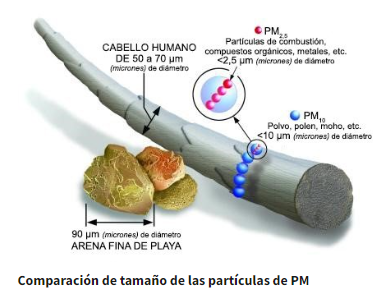
\includegraphics[scale=1.2]{cabello}
\end{center}
\centering
\caption{Comparación del tamaño del material particulado.}
\label{cabello}
\end{figure}


De acuerdo con la organización mundial de la salud (2018), la contaminación del aire aumenta cada día más, en paises de bajo y medio ingreso, afectando la salud de los niños, principalmente. En el año 2016 las muertes de niños a causa de enfermedades respiratorias como consecuencia de la contaminación atmosférica, ascendieron a las $600.000$ en todo el mundo. 

En \cite{OMS}, se menciona que una de las principales causas de que los niños sean los que mas sufren por la contaminación atmosférica, es porque ellos respiran mas rápido que los adultos, razon por la cual, absorven mas micropartículas. 

A causa de lo anterior y de los descubrimientos sobre cancer de pulmón causados por el material partículado, en \cite{IARC} la organización mundia de la salud, establece algunas medidas que se deben tomar en todos los países para contrarestar esta situación y evitar que la contaminación continue cobrando vidas. 

Estas medidas establecidas estan relacionadas con la toma de acciones y la creación de políticas públicas que eviten la contaminación y reglamenten el uso adecuado de los recursos en las industrias públicas y privadas para disminuir su aporte de contaminación. 

\subsection{Ozono ($O_3$)} El Ozono, es un gas, que al rededor del ser humano puede generar daños a la salud respiratoria. Exposiciones por horas continuas a altas concentraciones de este contaminante pueden reducir la capacidad pulmonar, inflamar las vías respiratorias, producir infecciones respiratorias, etc. 

\section{Reglamentación}
Para el presente análisis, es necesario estudiar la reglamentación establecida por el ministerio de ambiente y desarrollo sostenible de Colombia, el cual, en la resolución N° $2254$ del 1 de noviembre de 2017: \textit{Por la cual se adopta la norma del aire y se dictan otras disposiciones,} establece que a partir del 1 de julio del 2018 los niveles máximos permisibles de contaminantes criterio en el aire son los que se presentan en la tabla \ref{nivelesperm}:
\begin{table}[!h]
\begin{center}
\begin{tabular}{|c|c|}
\hline
Contaminante & Nivel máximo permisible \\
\hline \hline
$PM_{10}$ &$ 75\mu g /m^3$ \\ \hline
$PM_{2.5}$ & $ 37 \mu g /m^3$  \\ \hline
$0_3$ & $100 ppb$ \\\hline
\end{tabular}
\caption{Normativa establecida en la resolución $2254$ para cada uno de los tres contaminantes.}
\label{nivelesperm}
\end{center}
\end{table}

\section{Datos de los tres contaminantes:}

Estos 1096 datos diarios de los tres contaminantes, fueron obtenidos a partir de los datos horarios registrados en las 13 estaciones de monitoreo de calidad del aire de Bogotá. Para el caso del $PM_{10}$ y $PM_{2.5}$ se determinaron promedios por cada 24 horas y de estos promedios se elegía el valor máximo; para el caso del $O_3$, algo similar, solo que, en lugar de promedio se tomo el máximo de cada periodo de un día. 

A continuación, se verifica mediante el software R, la cantidad de veces que estos umbrales se rebasan en los 1096 días de los años 2018 a 2020, en la figura \ref{seriesdet} se muestran las series de tiempo que describen el comportamiento diario de los contaminantes durante los tres años analizados.

Para el caso del PM 10, sucede algo particular y es que sus valores máximo y mínimo suceden en el mismo mes, aquí se observa que el día 24 de junio del 2020, se presentó una medición de $172.37$, sobrepasando considerablemente el máximo permitido y para el día 15 de junio del mismo año, se obtuvo una medición mínima en los tres años de $14.06$. Para este contaminante, se observaron un total de $318$ rebases.

En cuanto al material particulado $PM_{2.5}$ se observó que este rebasaba los umbrales permitidos un $30,3\%$ de veces, con un total de $332$ días en los que la norma no se esta cumpliendo, se puede observar en la figura \ref{seriesdet} que el día 28 de marzo del 2019, este contaminante sobrepasó el umbral permitido en más del $200\%$. 


Para la serie de tiempo que muestra los máximos diarios de concentración de Ozono en la ciudad de Bogotá, se debe tener en cuenta que, en la resolución número $2254$ del ministerio de ambiente y desarrollo sostenible, se presenta el umbral de este contaminante medido en $\mu g / m^3$ y en las estaciones de monitoreo se recibe la información en partes por billón $(ppb)$, de manera que se debe realizar la revisión de rebases, cuando los datos recogidos superen el valor aproximado de $50,9375 \text{ } ppb$ que corresponde a los $100 \mu g / m^3$ que establece la norma, esto nos da un total de 219 rebases en los tres años analizados. 



\begin{figure}[!h]
\begin{center}
\includegraphics[scale=1.5]{seriesdetiempo}
\end{center}
\centering
\caption{Niveles de concentración diaria de contaminantes $O_3$, $PM_{10}$ y $PM_{2.5}$, la recta horizontal representa el umbral máximo permitido por las autoridades ambientales en Colombia.}
\label{seriesdet}
\end{figure}

En la tabla \ref{rebasesporcontaminante} se muestra un resumen de los rebases obtenidos para cada uno de los contaminantes de interés, teniendo en cuenta que para el $O_3$ los rebases se determinaron sobre un valor de $50.93$ luego de realizar la respectiva conversión de partes por billón a $\mu g/m^3$. 

En la figura \ref{mediasacum} se presentan los graficos de las medias acumuladas de los rebases de los umbrales máximos permitidos. En ellos se puede evidenciar que hubo meses en los cuales no se presentaron rebases, esto se observa cuando las gráficas se muestran como una constante, un ejemplo es el caso del Ozono, en los meses comprendidos entre marzo y julio de 2018, no hubo ni un solo rebase, así como también entre los meses de abril y agosto del año 2019. De esta misma manera ocurre con los otros dos contaminantes, sin embargo es el Ozono, en el cual los periodos en los que no se rebasan los umbrales son mas extensos. 



\begin{table}[!h]
\begin{center}
\begin{tabular}{|c|c|c|c|}
\hline
Contaminante & Umbral & Rebases & Porcentaje \\
\hline \hline
$PM_{10}$ & $70\mu g /m^3$ &  318  & $29\%$ \\ \hline
$0_3$& $100 ppb$ &  219 & $20\%$  \\ \hline
$PM_{2.5}$ & $37\mu g /m^3$ & 332 & $30.3 \%$  \\ \hline
\end{tabular}
\caption{Número de rebases de cada contaminante.}
\label{rebasesporcontaminante}
\end{center}
\end{table}


 
\begin{figure}[!t]
\begin{center}
\includegraphics[scale=1.5]{mediasacumuladas}
\end{center}
\centering
\caption{Media acumulada observada del número de excedencias para cada uno de los tres contaminantes.}
\label{mediasacum}
\end{figure}

Para estudiar el número de rebases de los umbrales ambientales, se considera un proceso de Poisson con función de intensidad $\lambda (t),$ con la forma Weibull, que depende de los parámetros $\a$ y $\b$ de acuerdo con la siguiente expresión: 

$$\lambda(t)=\frac{\a}{\b}\left(\frac{t}{\b}   \right)^{\a -1}, \a, \b >0 \text{ y } t \geq 0 $$ 

A partir de esta expresión se construyen las funciones de riesgo para cada uno de los modelos, teniendo en cuenta que cuando el parámetro $\a<1$ la función es decreciente, si $\a>1$  será creciente y constante cuando $\a=1$
\newpage
\section{Sin puntos de cambio}

Para estimar los parámetros de este modelo, se realizaron $20.000$ iteraciones y se eliminaron $2.000$ de ellas. En esta implementación se encontró que para el $PM_{10}$, los parámetros son $\a=0.89$ y $\b=1.76$, lo cual indica que la función de riesgo será decreciente, esto lo que quiere decir, es que el número de rebases tiende a disminuir con el paso del tiempo. 

Para el caso del $PM_{2.5}$, se obtuvo: $\a=1.16$ y $\b=1.75$ y para el ozono, $\a=1.21$ y $\b=13.37$, estos últimos valores de $\a$ demuestran que las funciones son crecientes, de manera que con el paso del tiempo los niveles de contaminación de $PM_{2.5}$ y $O_3$ aumentarán.  

En ausencia de puntos de cambio, se determinaron los siguientes parámetros $\a$  y  $\b$ con los cuales se podrán construir las funciones de riesgo acumuladas: 

\begin{table}[!h]
\centering
\begin{tabular}{|l|l|l|l|l|l|}
\hline
& \multicolumn{5}{c|}{Información estadística} \\
\cline{2-6}
& Parámetros & dist. inicial  & Media & sd  &   intervalo $95 \%$\\
\hline \hline
\multirow{2}{1.5cm}{$PM_{10}$} & $\a_1$ & $unif(1,3)$ & $0.89$ & $0.05$ & $(0.79;0.99)$ \\ \cline{2-6}
& $\b_1$& $unif(1,10)$ & $1.76$ & $0.65$ & $(0.77;3.28)$\\  \cline{1-6}
\multirow{2}{1.5cm}{$PM_{2.5}$} & $\a_1$ & $dunif(1,2.8)$& $1.25$ & $0.02$ & $(1.22;1.31)$\\ \cline{2-6}
& $\b_1$ & \multicolumn{1}{c|}{$dunif(10;100)$} & $10.85$ & $0.83$ & $(10.02;13.06)$\\ \cline{1-6}
\multirow{2}{1.5cm}{$O_3$} & $\a_1$ & $dunif(1,5.99)$ & $1.21$& $0.03$ & $(1.16;1.29)$\\ \cline{2-6}
&$\b_1$ & \multicolumn{1}{c|}{$dunif(11.9,141)$} & $13.37$ & $1.41$ & $(11.94;17.12)$\\ \cline{1-6}
\end{tabular}
\caption{Información estadística de cada modelo sin puntos de cambio.}
\label{infoestad}
\end{table}



Teniendo estos parámetros,en la figura \ref{riesgo} se presentan las diferentes funciones de riesgo $\lambda (t)$ para cada uno de los tres contaminantes, esto sin tener en cuenta algún punto de cambio. 



\begin{figure}[!h]
\begin{center}
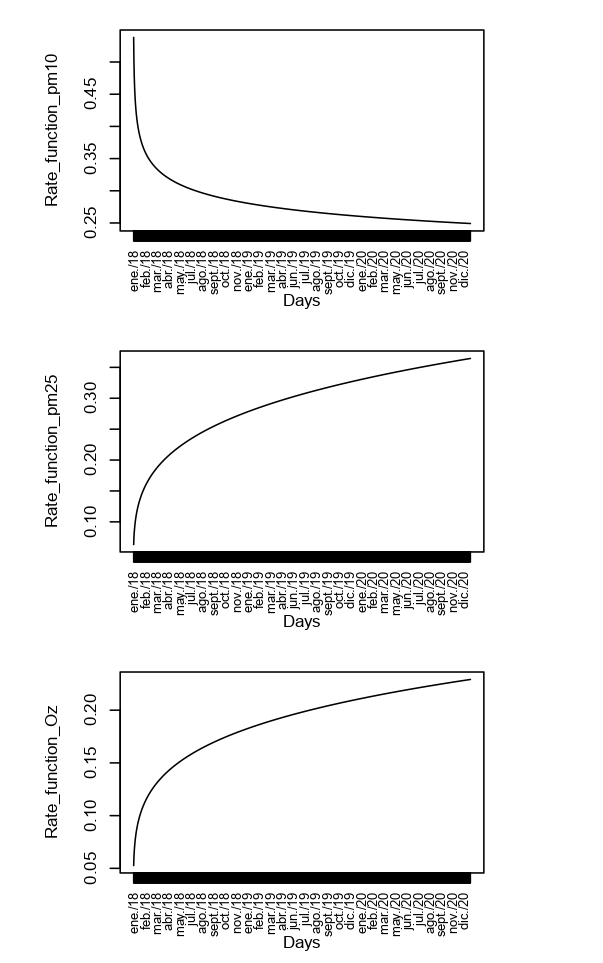
\includegraphics[width=13cm]{RIESGOSPC}
\end{center}
\centering
\caption{ Función de riesgo $\lambda (t) $, estimada para el modelo en ausencia de puntos de cambio.  }
\label{riesgo}
\end{figure}


El comportamiento de los rebases de cada contaminante se puede observar a través de la función de media acumulada $m(t)$, observada y estimada. En nuestro caso se observa en la figura  \ref{mediasacumcomp}, la función de media acumulada estimada en color azul, frente a lo estimado con un intervalo de confianza del $95\%$ de credibilidad, lo cual se representa mediante las lineas verdes, buscando hacer un ajuste y contraste con lo observado, que se presenta de color negro.



\begin{figure}[h!]
\begin{center}
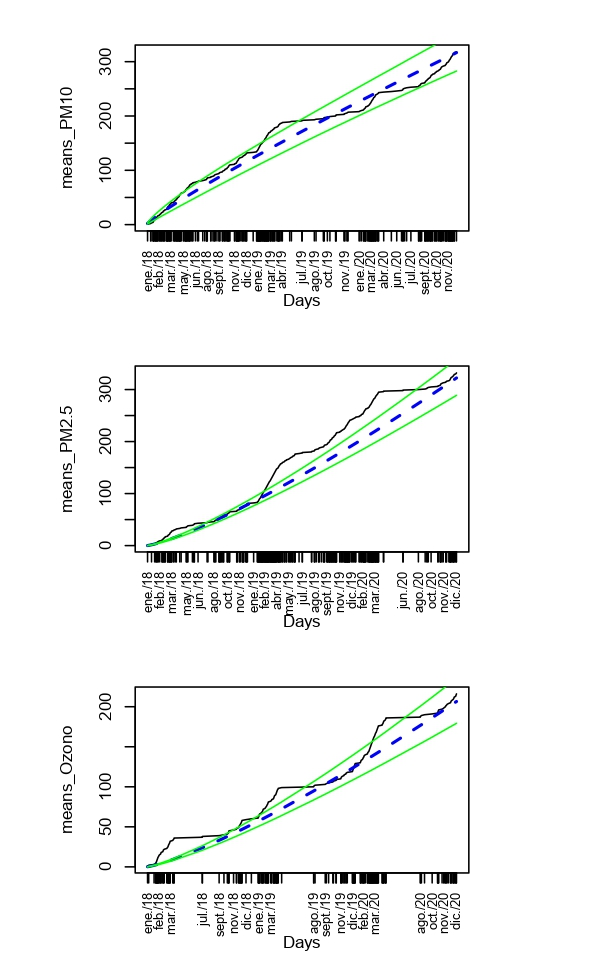
\includegraphics[width=11cm]{MEANSSPC}
\end{center}
\centering
\caption{ Función de media acumulada (azul), junto con los intervalos de confianza estimados con un 95\% de confianza (verde) y los datos observados (negro).  }
\label{mediasacumcomp}
\end{figure}



Se puede observar, que para el caso del $PM_{10}$, el modelo inicia con un buen ajuste, sin embargo para los meses posteriores a enero del 2019, se ve un desajuste considerable. Caso contrario el del $PM_{2.5}$ cuya estimación no es favorable en la mayoría de los meses estudiados, al igual que en el caso del ozono, en el cual se ve un buen ajuste durante los tres primeros meses y durante el mes de abril del año 2020. 



\newpage


\section{Un punto de cambio}
 

Este primer punto se encontró gráficamente, observando cambios en la figura \ref{mediasacum}, e identificando acontecimientos sucedidos en las fechas donde se observan dichos cambios. Estos puntos pueden ser aproximadamente los siguientes: 
$\tau_1=380$, $\tau_2=415$ y $\tau_3=115$, para $PM_{10}$, $PM_{2.5}$ y $O_3$ respectivamente.  



Para estos modelos se tendrán en cuenta dos tramos de las gráficas de medias acumuladas, que estarán determinados por el punto de cambio elegido. Es decir que antes de cada punto de cambio se determinarán un $\a$ y un $\b$ y para después del punto de cambio, otros $\a$ y $\b$ diferentes. Estos modelos se presentan en la figura \ref{mediasacumupc}

\begin{figure}[h!]
\begin{center}
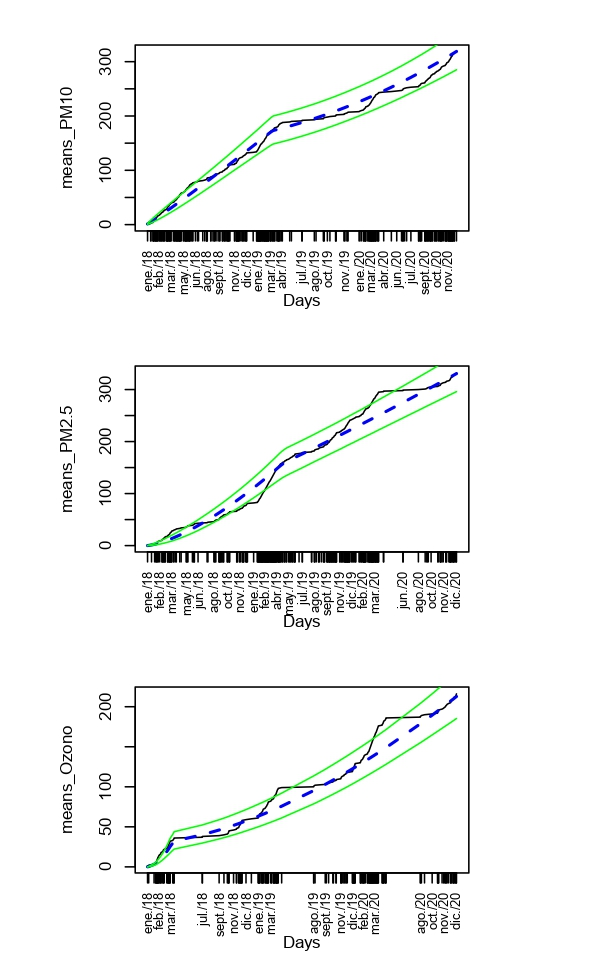
\includegraphics[width=11cm]{MEANSUPC}
\end{center}
\centering
\caption{ Función de media acumulada (azul), junto con los intervalos de confianza estimados con un 95\% de confianza (verde) y los datos observados (negro), para un punto de cambio.  }
\label{mediasacumupc}
\end{figure}


Los parámetros estimados para este modelo, fueron obtenidos realizando 20.000 iteraciones, al igual que en sin un punto de cambio. Se observa aquí que los parámetros $\a$ para el contaminante $PM_{10}$ fueron mayores que $1$, lo que indica que el comportamiento del contaminante, tiende a  aumentar su concentración con el paso del tiempo. De la misma forma, para los contaminantes  $PM_{2.5}$ y $O_3$ ambos parámetros son mayores que $1$, de manera que, así como se observó en el modelo sin puntos de cambio, antes y después del punto establecido, los contaminantes mantienen la predicción de aumento con el paso del tiempo. Estos resultados se encuentran resumidos en la tabla \ref{infoestadupc} y la gráfica correspondiente a las funciones de riesgo se muestran en la figura 
 


\begin{table}[!h]
\centering
\begin{tabular}{|l|c|l|l|l|l|}
\hline
& \multicolumn{5}{c|}{Información estadística} \\
\cline{2-6}
& Parámetros & dist. inicial  & Media & sd  &   intervalo $95 \%$\\
\hline \hline
\multirow{5}{1.5cm}{$PM_{10}$} & $\tau_1$ & $dunif(350,450))$ & $445.13$ & $ 4,34 $ & $(432.79;449.89)$ \\ \cline{2-6}
& $\a_1$& $dunif(1, 3)$ & $1.06$ & $0.08$ & $(0.91;1.21)$\\  \cline{2-6}
& $\b_1$& $dunif(1,100)$ & $3,63$ & $1.25$ & $(1.56;6.48)$\\  \cline{2-6}
& $\a_2$& $dunif(1,3)$ & $2.01$ & $0.13$ & $(1.68; 2.17)$\\  \cline{2-6}
& $\b_2$& $dunif(1,100)$ & $84.23$ & $13.54 $ & $(49.34;99.55)$\\  \cline{1-6}
\multirow{5}{1.5cm}{$PM_{2.5}$} & $\tau_1$ & $dunif(350,500)$& $483.53$ & $9.44$ & $(465.86;498.37)$\\ \cline{2-6}
& $\a_1$& $dunif(1,2.5)$ & $1.45$ & $0.11$ & $(1.25;1.68)$\\  \cline{2-6}
& $\b_1$& $dunif(6.4, 78.5)$ & $14.90$ & $4.04$ & $(8.19;23.72)$\\  \cline{2-6}
& $\a_2$& $dunif(1,2.5))$ & $1.28$ & $0.15$ & $(1.10;1.65)$\\  \cline{2-6}
& $\b_2$& $dunif(6.4, 78.5)$ & $15.21$ & $9.15$ & $(6.58;41.13)$\\  \cline{1-6}
\multirow{5}{1.5cm}{$O_3$} & $\tau_1$ & $dunif(50,200)$ & $96.40$& $5.89$ & $(83,56;104,13)$\\ \cline{2-6}
& $\a_1$& $dunif(1, 6)$ & $1.83$ & $0.17$ & $(1.57;2.24)$\\  \cline{2-6}
& $\b_1$& $dunif(11.9, 141)$ & $14.69$ & $2.35$ & $(11.99; 20.71)$\\  \cline{2-6}
& $\a_2$& $dunif(1, 5.9)$ & $1.66$ & $0.15$ & $(1.38;1.97)$\\  \cline{2-6}
& $\b_2$& $dunif(11.9, 141)$ & $48.45$ & $13.98$ & $(24.36;79.27)$\\  \cline{1-6}
\end{tabular}

\caption{Información estadística de cada modelo con un  punto de cambio.}
\label{infoestadupc}
\end{table}


\begin{figure}[hbt!]
\begin{center}
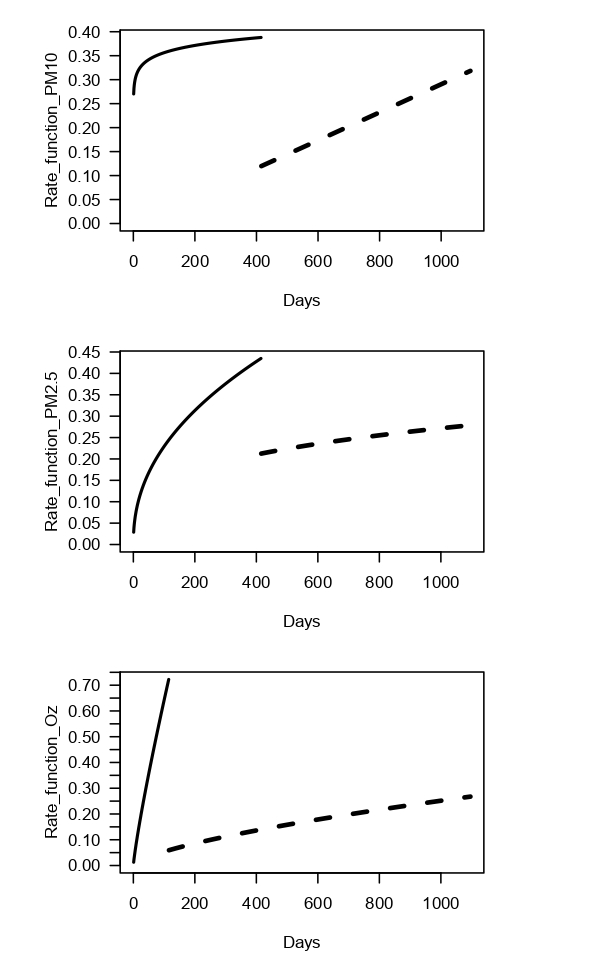
\includegraphics[width=13cm]{RIESGOUPC}
\end{center}
\centering
\caption{ Función de riesgo $\lambda (t)$, estimada para el modelo construido bajo un punto de cambio.   }
\label{rate_upc}
\end{figure}

\newpage
\section{Dos puntos de cambio:}

Al igual que en la sección anterior, de manera que se eligieron dos puntos de cambio que visualmente parecen ser representativos y en los cuales, según las fechas, hubo implementaciones de normas para combatir la contaminación ambiental, estos son por ejemplo, para el caso del contaminante $PM_{10}$ los días $\tau_1=446$ y $\tau_2=754$ aproximadamente, para el $PM_{2.5}$ los días $\tau_1=460$ y $\tau_2=821$ y para el $O_3$ los días $\tau_1=99$ y $\tau_2=468$ 
Abril del 2018 \cite{res2018}, Marzo del 2019\cite{barreto}, Enero del 2020 y marzo del 2020 \cite{dec2020} y \cite{dec20202}. 
\begin{table}[!h]
\centering
\begin{tabular}{|l|c|l|l|l|l|}
\hline
& \multicolumn{5}{c|}{Información estadística} \\
\cline{2-6}
& Parámetros & dist. inicial  & Media & sd  &   intervalo $95 \%$\\
\hline \hline
\multirow{8}{1.5cm}{$PM_{10}$} & $\tau_1$ & $dunif(250,450))$ & $446.22$ & $3.63 $ & $(437.42;449.93)$ \\ \cline{2-6}
& $\tau_2$& $dunif(700, 900)$ & $754.19$ & $18.09$ & $(726.01;777.40)$\\  \cline{2-6}
& $\a_1$& $dunif(0,3)$ & $1.07$ & $0.08$ & $(0.92;1.23)$\\  \cline{2-6}
& $\b_1$& $dunif(0,100)$ & $3.71$ & $1.32$ & $(1.61; 6.74)$\\  \cline{2-6}
& $\a_2$& $dunif(0,3)$ & $1.33$ & $0.32$ & $(0.74; 1.23)$\\  \cline{2-6}
& $\b_2$& $dunif(0,100)$ & $37.39$ & $27.07$ & $(1.43; 94.18)$\\  \cline{2-6}
& $\a_3$& $dunif(0,3)$ & $1.89$ & $0.26$ & $(1.24; 2.21)$\\  \cline{2-6}
& $\b_3$& $dunif(0,100)$ & $66.40$ & $24.67 $ & $(11.47;98.78)$\\  \cline{1-6}
\multirow{8}{1.5cm}{$PM_{2.5}$} & $\tau_1$ & $dunif(300,500)$& $460.23$ & $43.77$ & $(368.97;498.00)$\\ \cline{2-6}
& $\tau_2$& $dunif(698,898)$ & $821.60$ & $3.36$ & $(817.50;829.87)$\\  \cline{2-6}
& $\a_1$& $dunif(1,3.5)$ & $1.37$ & $0.18$ & $(1.02;1.67)$\\  \cline{2-6}
& $\b_1$& $dunif(1,100)$ & $13.19$ & $4.94$ & $(5.02;23.27)$\\  \cline{2-6}
& $\a_2$& $dunif(1,3.5)$ & $2.05$ & $0.47$ & $(1.06;2.50)$\\  \cline{2-6}
& $\b_2$& $dunif(1,100)$ & $66$ & $33.44$ & $(2.94;99.07)$\\  \cline{2-6}
& $\a_3$& $dunif(1,3.5))$ & $1.66$ & $0.19$ & $(1.18;1.92)$\\  \cline{2-6}
& $\b_3$& $dunif(1,100)$ & $71.063$ & $22.56$ & $(18.20;99.07)$\\  \cline{1-6}
\multirow{8}{1.5cm}{$O_3$} & $\tau_1$ & $dunif(50,200)$ & $99.18$& $1.81$ & $(97.51;104,09)$\\ \cline{2-6}
& $\tau_2$& $dunif(350,500)$ & $468.10$ & $4.02$ & $(462.65;479.67)$\\  \cline{2-6}
& $\a_1$& $dunif(1,6)$ & $1.83$ & $0.16$ & $(1.57;2.20)$\\  \cline{2-6}
& $\b_1$& $dunif(12,141)$ & $14.64$ & $2.25$ & $(12.08;20.35)$\\  \cline{2-6}
& $\a_2$& $dunif(1,6)$ & $3.30$ & $0.19$ & $(2.86;3.59)$\\  \cline{2-6}
& $\b_2$& $dunif(12, 141)$ & $131.81$ & $8.48$ & $(109.41; 140.74)$\\  \cline{2-6}
& $\a_3$& $dunif(1, 6)$ & $2.12$ & $0.21$ & $(1.62;2.41)$\\  \cline{2-6}
& $\b_3$& $dunif(12, 141)$ & $107.05$ & $25.23$ & $(47.89;139.68)$\\  \cline{1-6}
\end{tabular}
\caption{Información estadística de cada modelo con dos puntos de cambio.}
\label{infoestaddpc}
\end{table}

Los resultados de utilizar estos puntos de cambio correspondientes a las siguientes fechas aproximadas, Abril del 2018, Marzo del 2019, Enero del 2020 y marzo del 2020, se presentan en la figura \ref{mediasacumdpc}, aquí se observa la manera en que el ajuste es cada vez mas perfecto. 

\begin{figure}[h!]
\begin{center}
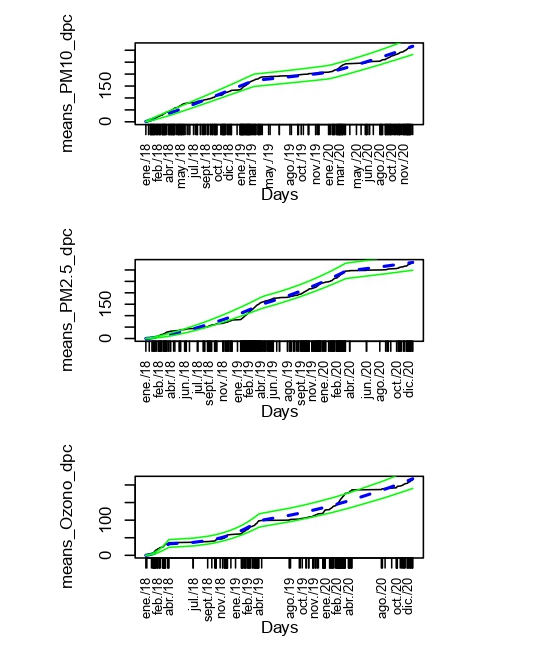
\includegraphics[width=12cm]{MEANSDPC}
\end{center}
\centering
\caption{ Función de media acumulada (azul), junto con los intervalos de confianza estimados con un 95\% de confianza (verde) y los datos observados (negro), para dos puntos de cambio.  }
\label{mediasacumdpc}
\end{figure}

Con los parámetros obtenidos para cada uno de los intervalos de tiempo determinados por los dos puntos de cambio, tabla \ref{infoestaddpc}, se determinan las funciones de riesgo que describen el comportamiento de los tres contaminantes en cada periodo de tiempo. 
En la figura \ref{rate_dpc} se observa qué las medidas implementadas por la alcaldía de Bogotá funcionan, pero de manera momentanea, por ejemplo para el caso del $PM_{10}$ se observa como los niveles de contaminación en el primer tramo son altos, y luego para el segundo momento disminuyen y tienden a permanecer 'constantes'; sin embargo para el momento que sigue, la implementación de restricciones de movilidad y control de contaminantes en grandes industrias de febrero y marzo del 2020, cuando se declaró emergencia ambiental, ocasionaron, según la grafica, que el nivel de concentración de $PM_{10}$ empezara a aumentar y a mostrar una tendencia creciente. 

\begin{figure}[hbt!]
\begin{center}
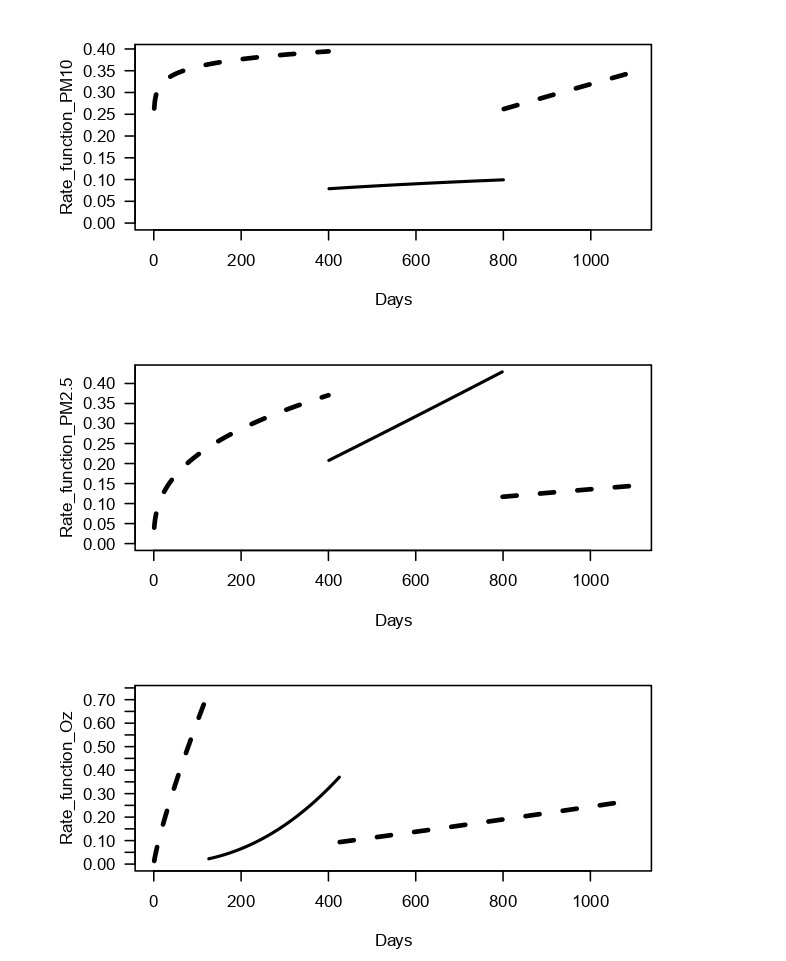
\includegraphics[width=13cm]{RATEDPC}
\end{center}
\centering
\caption{ Función de riesgo $\lambda (t)$, estimada para el modelo construido bajo dos puntos de cambio.   }
\label{rate_dpc}
\end{figure}



\newpage

\section{Política pública:}

Como ya se mencionó, los puntos de cambio de los modelos construidos se determinaron principalmente con ayuda de las gráficas de las medias acumuladas de cada uno de los contaminantes, para validar estos puntos, una posibilidad es identificar algunas de las estrategias del gobierno nacional para mitigar la contaminación ambiental durante estas fechas.
Uno de los insumos mas importantes que permite identificar esto, es el \textit{plan decenal de desconaminación del aire de Bogotá} que se elabora cada 10 años y al cual se le realizan revisiones periódicas para verificar su alcance y cumplimiento. 
El documento que compete a esta investigación, es el elaborado para la década del 2010 al 2020 \cite{plandecenal}, en el cual, al igual que en la anterior década, se centran en la implementación de las siguientes acciones para mejorar la calidad del aire: 

\begin{itemize}
\item Pico y placa ambiental.
\item Pico y placa de movilidad. 
\item Mejoramiento del ACPM.
\item Operativos en Vía.
\item Control a fuentes industriales.
\item Inventarios de emisiones. 
\end{itemize}

Estas acciones, se organizaron para ser implementadas durante los 10 años en diferentes etapas, para el caso del periodo de tiempo que se esta teniendo en cuenta en el presente documento, las acciones planteadas son, para el 2019 y 2020 únicamente, en el sector industrial, se estableció el proyecto \textit{Uso de sistemas de control
de emisiones}, para los años 2012 al 2020, en cuestiones de transporte, se debían implementar los proyectos \textit{Uso de sistemas de control de emisiones en vehículos de transporte de carga}, y \textit{Uso de sistemas de control 
de emisiones en motocicletas} y para el periodo comprendido entre 2011 y 2020 el proyecto \textit{Implementación del sistema
integrado de transporte
público}. 

En la ciudad de Bogotá, se han reducido los niveles de concentración de $PM_{10}$ y $PM_{2.5}$ entre los años de 2012 y 2017 gracias a las propuestas implementadas en el plan decenal de decontaminación del aire para Bogotá, como por ejemplo la integración del transporte público SITP y la descontinuación de algunas busetas que no cumplían con las características establecidas para contrarrestar la contaminación; el seguimiento y control en la industria, aumento en los días sin carro, entre otras.
Puntualmente, para el caso del $PM_{10}$ y el $PM_{2.5}$ su primer punto de cambio ocurre al rededor del dato 400, el cual corresponde a una fecha aproximada al 4 de febrero del 2019, este cambio se puede explicar en parte, por la resolución 383 del año 2019 \cite{res2019}, en la cual se declara alerta amarilla porque el material particulado excede los umbrales máximos permitidos. Así mismo, para el caso del Ozono, sucede algo similar solo que su primer punto de cambio ocurre en marzo del 2018, cuando en la resolución 831 de 2018 \cite{res2018} también es decretada la alerta amarilla por contaminación ambiental y se establecen algunas restricciones en la ciudad de Bogotá, como por ejemplo establecer  restricciones en el sector de transporte y movilidad y restringir la operaciones de fuentes fijas industriales que operan con combustibles sólidos y líquidos. 

En el año 2020, para los meses de febrero y marzo se decretó  alerta amarilla en la ciudad de Bogotá, por medio del decreto 077 del 4 de marzo de 2020 \cite{dec20202} y \cite{dec2020}, el cual esta relacionado con la restricción de vehiculos de carga, dado que los niveles de concentración de material particulado se encontraban elevados en algunas estaciones de monitoreo y por esta fecha se estaban presentando incendios forestales, aun cuando la movilidad se empezaba a restringir a causa de la pandemia ocasionada por el Covid 19. 
 

\chapter{Diagnóstico de convergencias}

\section{Sin puntos de cambio}
De acuerdo a las simulaciones generadas para cada modelo, se realizaron los análisis de convergencia correspondientes obteniendo resultados favorables que indican que el modelo muestra buenos resultados pues los parámetros cumplen la mayoría de los criterios, esto se muestra en las tablas \ref{converpm10spc}, \ref{converpm25spc} y 
\ref{converozono}. 

En todos los casos, para el criterio de convergencia propuesto en Geweke (1992), se observa que cada una de las pruebas aplicadas a las cinco cadenas realizadas, satisface la condición de que el valor $Z$ calculado, se encuentre entre el intervalo $(-2,2)$ esto da un buen indicio sobre la convergencia de los parámetros. 

Por otra parte, el criterio Heidelberg-Welch de estacionalidad fue  satisfactoria para todas las cadenas, por lo cual se identifica si el ancho medio para cada una de ellas es menor que $\varepsilon =0.1 $, y esto, en efecto es cierto en todas las cadenas realizadas para los tres contaminantes. 

Y finalmente el criterio de Gelman Rubin, menciona que valores cercanos a 1, indicarían una posible convergencia y en cada uno de los tres contaminantes su valor fue cercano a 1. De esta manera, cumpliendo la mayoría de condiciones de cada uno de los criterios de convergencia estudiados, se puede afirmar con seguridad que los parámetros estimados  funcionan adecuadamente. 


%%SPC-CONVERGENCIA-PM10

\begin{table}[!h]
\centering
\begin{tabular}{|l|c|l|l|l|l|l|}
\hline
& \multicolumn{6}{|c|}{Diagnóstico de convergencia} \\
\cline{2-7}
& Parámetro & cadena 1  & cadena 2  & cadena 3 & cadena 4 & cadena 5	 \\
\hline \hline
\multirow{2}{2.5cm}{Geweke} & $\a$ & $0.03089$ & $1.585$ & $-1.765$ & $-0.5473$  & $-0.1294$\\ \cline{2-7}
& $\b$& $-0.24968 $ & $1.296$ & $-1.641$ & $-0.3181$ & $-0.23$\\
  \cline{1-7}
\multirow{2}{2.5cm}{Raftery - Lewis} & $\a$ & $16.9$& $ 16.3$ & $18.7$ & $22.5 $ & $  16.7 $\\ \cline{2-7}
& $\b$ & \multicolumn{1}{l|}{$16.8$} & $26.7$ & $ 17.3$ & $22.0$ & $18.2$ \\ \cline{1-7}
\multirow{2}{2.5cm}{H-W Estacionalidad} & $\a$ & $0.877$ & $0.642$ & $0.903$ & $0.916$ & $0.680$ \\ \cline{2-7}
&$\b$ & \multicolumn{1}{l|}{$0.890$} & $0.598$ &  $ 0.826$ & $0.984$ & $0.747 $ \\ \cline{1-7}
\multirow{2}{2.5cm}{H-W $1/2$ Ancho} & $\a$ & $0.00107$ & $ 0.00106$ & $ 0.00112$ & $0.000986 $  & $ 0.000891  $  \\ \cline{2-7}
&$\b$ & \multicolumn{1}{l|}{$0.02705  $} & $0.02698$ & $0.02746  $ & $0.024899$ & $0.022256$ \\ \cline{1-7}

\multirow{2}{2.5cm}{Gelman - Rubin} & $\a$ & \multicolumn{5}{|c|}{1.00}\\ \cline{2-7}
&$\b$ &  \multicolumn{5}{|c|}{1.00} \\ \cline{1-7}



\end{tabular}
\caption{Información de convergencia para el modelo $PM_{10}$, sin puntos de cambio. H-W=Heidelberger-Welch}

\label{converpm10spc}
\end{table}





%%SPC-CONVERGENCIA-PM25

\begin{table}[!h]
\centering
\begin{tabular}{|l|c|l|l|l|l|l|}
\hline
& \multicolumn{6}{|c|}{Diagnóstico de convergencia} \\
\cline{2-7}
& Parámetro & cadena 1  & cadena 2  & cadena 3 & cadena 4 & cadena 5	 \\
\hline \hline
\multirow{2}{2.5cm}{Geweke} & $\a$ & $0.0959$ & $0.5630$ & $-1.785$ & $-1.455$  & $ -0.2081$\\ \cline{2-7}
& $\b$& $0.1362$ & $0.4231$ & $-1.836$ & $-1.423 $ & $-0.1948$\\
  \cline{1-7}
\multirow{2}{2.5cm}{Raftery - Lewis} & $\a$ & $2.51 $& $  1.85$ & $2.50$ & $2.56  $ & $  2.56  $\\ \cline{2-7}
& $\b$ & \multicolumn{1}{l|}{$ 2.13$} & $2.41$ & $2.43$ & $2.29	 $ & $2.34  $ \\ \cline{1-7}
\multirow{2}{2.5cm}{H-W Estacionalidad} & $\a$ & $0.229  $ & $0.764 $ & $0.795$ & $0.484$ & $0.0534$ \\ \cline{2-7}
&$\b$ & \multicolumn{1}{l|}{$0.308 $} & $  0.507$ &  $ 0.776 $ & $ 0.474$ & $ 0.8327 $ \\ \cline{1-7}
\multirow{2}{2.5cm}{H-W $1/2$ Ancho} & $\a$ & $0.00291$ & $0.00253$ & $0.00253$ & $0.00232 $  & $0.00246 $  \\ \cline{2-7}
&$\b$ & \multicolumn{1}{l|}{$0.09838  $} & $0.08906$ & $0.08830 $ & $ 0.07683$ & $0.07932 $ \\ \cline{1-7}

\multirow{2}{2.5cm}{Gelman - Rubin} & $\a$ & \multicolumn{5}{|c|}{1}\\ \cline{2-7}
&$\b$ &  \multicolumn{5}{|c|}{1} \\ \cline{1-7}



\end{tabular}
\caption{Información de convergencia para el modelo $PM_{2.5}$, sin puntos de cambio. H-W=Heidelberger-Welch}

\label{converpm25spc}
\end{table}




%%SPC-CONVERGENCIA-Ozono

\begin{table}[!h]
\centering
\begin{tabular}{|l|c|l|l|l|l|l|}
\hline
& \multicolumn{6}{|c|}{Diagnóstico de convergencia} \\
\cline{2-7}
& Parámetro & cadena 1  & cadena 2  & cadena 3 & cadena 4 & cadena 5	 \\
\hline \hline
\multirow{2}{2.5cm}{Geweke} & $\a$ & $0.7882$ & $0.2856 $ & $0.7351$ & $0.9028$  & $ -0.07696$\\ \cline{2-7}
& $\b$& $0.7052 $ & $0.2041$ & $0.9396$ & $0.8609$ & $-0.14975$\\
  \cline{1-7}
\multirow{2}{2.5cm}{Raftery - Lewis} & $\a$ & $ 1.72  $& $  1.67$ & $ 2.40$ & $1.94 $ & $ 1.80 $\\ \cline{2-7}
& $\b$ & \multicolumn{1}{l|}{$1.31$} & $1.26$ & $ 1.34 $ & $1.22 $ & $1.25$ \\ \cline{1-7}
\multirow{2}{2.5cm}{H-W Estacionalidad} & $\a$ & $0.408$ & $0.907 $ & $0.234$ & $ 0.351$ & $0.273$ \\ \cline{2-7}
&$\b$ & \multicolumn{1}{l|}{$0.4185$} & $ 0.924$ &  $ 0.113  $ & $0.374$ & $ 0.335  $ \\ \cline{1-7}
\multirow{2}{2.5cm}{H-W $1/2$ Ancho} & $\a$ & $0.00139$ & $0.00172$ & $0.00163$ & $0.0018 $  & $0.00151$  \\ \cline{2-7}
&$\b$ & \multicolumn{1}{l|}{$0.06699 $} & $0.08421$ & $0.07863$ & $ 0.0883$ & $0.07574 $ \\ \cline{1-7}

\multirow{2}{2.5cm}{Gelman - Rubin} & $\a$ & \multicolumn{5}{|c|}{1}\\ \cline{2-7}
&$\b$ &  \multicolumn{5}{|c|}{1.01} \\ \cline{1-7}

\end{tabular}
\caption{Información de convergencia para el modelo $O_3$, sin puntos de cambio. H-W=Heidelberger-Welch}
\label{converozono}
\end{table}

\section{Un punto de cambio}

El diagnóstico de convergencia para un punto de cambio, arrojó algunos resultados importantes que se deben mencionar. Iniciando con el criterio de Geweke (1992), este es satisfactorio en las cinco cadenas realizadas para el material particulado de $10\mu m$ de tamaño pues la comparación de los valores de las medias iniciales y finales de las cadenas, están entre -2 y 2. Para el caso del $PM_{2.5}$ se observa en la tabla \ref{convergencia_updc_pm25} que en algunas de las cadenas los valores no se encuentran entre -2 y 2, es el caso de los parámetros $\a_2$ y $\s_2$, en los cuales en dos y tres de las cadenas, respectivamente, los resultados se encuentran fuera del intervalo que se considera adecuado, sin embargo, estos números no son significativamente grandes. Para el caso del $O_3$ sucede lo mismo que en el $PM_{10}$ pues todos sus valores se encuentran dentro del intervalo que genera confianza, para poder hablar de estacionalidad y posiblemente de convergencia. 

Otro de los criterios que proporciona información sobre la convergencia de los parámetros es el test de estacionalidad de Heidelberger-Welch, pues los tres contaminantes lo pasaron, de manera que se procede a hacer la revisión del criterio del Ancho medio, el cual es satisfactorio para todos los parámetros $\a_1$ y $\a_2$ de los tres contaminantes, a excepción de una cadena del contaminante Ozono, sin embargo al ser solo una de cinco cadenas, no se tiene en cuenta, de forma que todos los parámetros $a_1$ y $a_2$ tienen una confirmación más de que tienen convergencia. Para el caso de los parámetros $\b_1$ y $\b_2$ este criterio, muestra que en algunas cadenas, sus valores no son menores a $0.1$, por tanto este criterio no es suficiente o de apoyo para argumentar convergencia de ellos, de forma similar con el parámetro $\tau$ en el caso de los tres contaminantes. 


Finalmente, para el caso de los modelos con un solo punto de cambio, se observó que el criterio Gelman- Rubin, es satisfactorio en los tres modelos, pues sus valores son cercanos a 1, toda la información anterior, se encuentra resumida en las tablas \ref{convergencia_updc_pm10}, \ref{convergencia_updc_pm25} y \ref{convergencia_updc_ozono}.


%%%%%TABLA DE CONV UPDC PM10


\begin{table}[!h]
\centering
\begin{tabular}{|l|c|l|l|l|l|l|}
\hline
& \multicolumn{6}{|c|}{Diagnóstico de convergencia} \\
\cline{2-7}
& Parámetro & cadena 1  & cadena 2  & cadena 3 & cadena 4 & cadena 5	 \\
\hline \hline
\multirow{5}{2.5cm}{Geweke} & $\a_1$ & $-0.2161$ & $-0.3797$ & $0.8125 $ & $-0.6749$  & $ 1.4716$\\ \cline{2-7}
& $\b_1$& $-0.2583 $ & $-0.3447$ & $0.8189$ & $-0.6263$ & $ 1.5856$\\
\cline{2-7}
& $\a_2$& $-0.3066 $ & $-0.1314 $ & $-1.1402$ & $ -0.4315$ & $1.0628$\\
\cline{2-7}
& $\b_2$& $-0.3165 $ & $0.1059$ & $-1.1862$ & $ -0.4369$ & $1.0672$\\
\cline{2-7}
& $\tau $& $-1.8701 $ & $-0.6091$ & $-1.4073$ & $0.1858$ & $-0.7393$\\
  \cline{1-7}
  \multirow{5}{2.5cm}{Raftery - Lewis} & $\a_1$ & $4.49$ & $5.25  $ & $2.88 $ & $2.67$  & $ 2.83 $\\ \cline{2-7}
& $\b_1$& $3.64 $ & $3.41 $ & $3.51$ & $3.01$ & $36.30 $\\
\cline{2-7}
& $\a_2$ & $18.60  $ & $30.10 $ & $13.60$ & $27.40$ & $4.69$\\
\cline{2-7}
& $\b_2$& $19.00 $ & $28.50$ & $13.80$ & $29.10 $ & $44.70$\\
\cline{2-7}
& $\tau $& $5.81 $ & $6.90$ & $6.85$ & $6.32 $ & $5.95$\\
  \cline{1-7}
  \multirow{5}{2.5cm}{H-W Estacionalidad} & $\a_1$ & $0.5609$ & $0.986 $ & $ 0.193$ & $0.186$  & $0.996$\\ \cline{2-7}
& $\b_1$& $0.5359  $ & $0.983   $ & $0.259$ & $0.212$ & $0.995$\\
\cline{2-7}
& $\a_2$& $0.0573 $ & $0.509$ & $0.651$ & $0.122$ & $0.653$\\
\cline{2-7}
& $\b_2$& $0.0973 $ & $0.593 $ & $0.639$ & $0.125$ & $0.646$\\
\cline{2-7}
& $\tau$& $0.4983 $ & $0.637 $ & $0.645$ & $0.327$ & $0.384$\\
  \cline{1-7}
  \multirow{5}{2.5cm}{H-W $1/2$ Ancho} & $\a_1$ & $0.00642$ & $0.00547 $ & $0.00679$ & $0.00705$  & $ 0.00758$\\ \cline{2-7}
& $\b_1$& $0.12170 $ & $0.10158$ & $0.12922$ & $0.13551$ & $0.14583$\\
\cline{2-7}
& $\a_2$& $0.01301 $ & $0.01932$ & $0.01404$ & $0.01324$ & $0.01780$\\
\cline{2-7}
& $\b_2$& $1.57577$ & $1.86337$ & $1.58302$ & $ 1.43715$ & $1.75334$\\
\cline{2-7}
& $\tau$& $0.16809  $ & $0.17736$ & $0.19509 $ & $0.18970$ & $0.21971$\\
  \cline{1-7}

\multirow{5}{2.5cm}{Gelman - Rubin} & $\a_1$ & \multicolumn{5}{|c|}{1.01}\\ \cline{2-7}
&$\b_1$ &  \multicolumn{5}{|c|}{1.01} \\ \cline{2-7}
&$\a_2$ &  \multicolumn{5}{|c|}{1.00} \\ \cline{2-7}
&$\b_2$ &  \multicolumn{5}{|c|}{1.00} \\ \cline{2-7}
&$\tau$ &  \multicolumn{5}{|c|}{1.00} \\ \cline{1-7}



\end{tabular}
\caption{Información de convergencia para el modelo $PM_{10}$, un punto de cambio. H-W=Heidelberger-Welch}
\label{convergencia_updc_pm10}
\end{table}


%%%%%TABLA DE CONV UPDC PM2.5


\begin{table}[!h]
\centering
\begin{tabular}{|l|c|l|l|l|l|l|}
\hline
& \multicolumn{6}{|c|}{Diagnóstico de convergencia} \\
\cline{2-7}
& Parámetro & cadena 1  & cadena 2  & cadena 3 & cadena 4 & cadena 5	 \\
\hline \hline
\multirow{5}{2.5cm}{Geweke} & $\a_1$ & $-0.2860$ & $-1.0051$ & $-17.774$ & $0.7692$  & $ -0.5075$\\ \cline{2-7}
& $\b_1$& $-0.3071 $ & $-0.9200$ & $0-12.524$ & $0.7046 $ & $ -0.5437 $\\
\cline{2-7}
& $\a_2$& $-2.6915 $ & $-3.8182 $ & $-1.997$ & $ -1.5921$ & $-1.3143 $\\
\cline{2-7}
& $\b_2$& $-2.5533$ & $-3.4243$ & $-4.756$ & $ -1.4134$ & $-1.2864$\\
\cline{2-7}
& $\tau $& $0.2518  $ & $-0.2185 $ & $-13.928$ & $0.6264$ & $1.0813$\\
  \cline{1-7}
  \multirow{5}{2.5cm}{Raftery - Lewis} & $\a_1$ & $13.60$ & $11.20  $ & $8.37  $ & $14.30$  & $  12.10 $\\ \cline{2-7}
& $\b_1$& $12.00 $ & $13.00 $ & $6.89$ & $11.40$ & $ 12.70 $\\
\cline{2-7}
& $\a_2$ & $4.54  $ & $3.14  $ & $4.19 $ & $2.85$ & $6.01 $\\
\cline{2-7}
& $\b_2$& $3.87 $ & $3.99$ & $2.60 $ & $29.10 $ & $5.17$\\
\cline{2-7}
& $\tau $& $7.59 $ & $4.33 $ & $14.40$ & $ 8.44 $ & $ 5.05$\\
  \cline{1-7}
  \multirow{5}{2.5cm}{H-W Estacionalidad} & $\a_1$ & $0.713$ & $0.2035  $ & $ 0.970$ & $0.381$  & $0.746$\\ \cline{2-7}
& $\b_1$& $0.714  $ & $0.2018  $ & $0.982$ & $0.361$ & $0.743$\\
\cline{2-7}
& $\a_2$& $0.161$ & $0.0714$ & $0.104$ & $0.445$ & $0.217$\\
\cline{2-7}
& $\b_2$& $0.203 $ & $0.1176 $ & $0.166$ & $0.647$ & $0.322$\\
\cline{2-7}
& $\tau$& $0.951 $ & $0.1457  $ & $0.989$ & $0.563$ & $0.328$\\
  \cline{1-7}
  \multirow{5}{2.5cm}{H-W $1/2$ Ancho} & $\a_1$ & $0.0161$ & $0.0150 $ & $0.0184$ & $0.0148 $  & $ 0.0167 $\\ \cline{2-7}
& $\b_1$& $0.5514 $ & $0.5158$ & $0.5726$ & $0.4953$ & $0.5719$\\
\cline{2-7}
& $\a_2$& $0.0239 $ & $0.0206$ & $0.0149$ & $0.0154$ & $0.0120$\\
\cline{2-7}
& $\b_2$& $1.4992$ & $1.1535$ & $0.8434$ & $ 0.8537$ & $0.6364$\\
\cline{2-7}
& $\tau$& $0.2058  $ & $0.1376$ & $5.0098 $ & $0.4146$ & $0.1456$\\
  \cline{1-7}

\multirow{5}{2.5cm}{Gelman - Rubin} & $\a_1$ & \multicolumn{5}{|c|}{1.03}\\ \cline{2-7}
&$\b_1$ &  \multicolumn{5}{|c|}{1.01} \\ \cline{2-7}
&$\a_2$ &  \multicolumn{5}{|c|}{1.03} \\ \cline{2-7}
&$\b_2$ &  \multicolumn{5}{|c|}{1.05} \\ \cline{2-7}
&$\tau$ &  \multicolumn{5}{|c|}{2.65} \\ \cline{1-7}



\end{tabular}
\caption{Información de convergencia para el modelo $PM_{2.5}$, un punto de cambio. H-W=Heidelberger-Welch}
\label{convergencia_updc_pm25}
\end{table}

%%%%%TABLA DE CONV UPDC OZONO 


\begin{table}[!h]
\centering
\begin{tabular}{|l|c|l|l|l|l|l|}
\hline
& \multicolumn{6}{|c|}{Diagnóstico de convergencia} \\
\cline{2-7}
& Parámetro & cadena 1  & cadena 2  & cadena 3 & cadena 4 & cadena 5	 \\
\hline \hline
\multirow{5}{2.5cm}{Geweke} & $\a_1$ & $0.1738$ & $-1.8966$ & $0.06743$ & $-3.1571$  & $-1.49105$\\ \cline{2-7}
& $\b_1$& $-0.7537$ & $-0.8614$ & $0.23790$ & $-2.5854$ & $ -1.0130 $\\
\cline{2-7}
& $\a_2$& $-1.7965$ & $-1.6817$ & $1.22712$ & $0.8546$ & $1.02269$\\
\cline{2-7}
& $\b_2$& $-1.9557$ & $-1.6606$ & $1.19464$ & $  0.8934$ & $ 0.9521$\\
\cline{2-7}
& $\tau $& $-0.7835   $ & $ 1.1726 $ & $-0.22160$ & $0.9531$ & $1.7600$\\
  \cline{1-7}
  \multirow{5}{2.5cm}{Raftery - Lewis} & $\a_1$ & $2.54$ & $2.67$ & $1.76  $ & $ 1.80$  & $  1.91 $\\ \cline{2-7}
& $\b_1$& $1.34  $ & $1.24 $ & $1.37$ & $11.40$ & $34.00$\\
\cline{2-7}
& $\a_2$ & $ 16.60 $ & $29.60  $ & $29.40 $ & $32.50$ & $ 2.51  $\\
\cline{2-7}
& $\b_2$& $20.70 $ & $ 18.50$  & $27.60$ & $35.70 $ & $42.00$\\
\cline{2-7}
& $\tau $& $2.90	$ & $ 2.52$ & $32.30$ & $ 2.11$ & $ 9.89$\\
  \cline{1-7}
  \multirow{5}{2.5cm}{H-W Estacionalidad} & $\a_1$ & $0.360$ & $0.000394 $ & $0.421$ & $0.0629$  & $0.222 $\\ \cline{2-7}
& $\b_1$& $0.193   $ & $0.070700  $ & $0.2334$ & $0.2334$ & $0.808 $\\
\cline{2-7}
& $\a_2$& $0.634 $ & $0.731613$ & $0.529$ & $0.6852$ & $0.340$\\
\cline{2-7}
& $\b_2$& $0.582 $ & $0.777112$ & $0.504$ & $ 0.6699$ & $0.286 $\\
\cline{2-7}
& $\tau$& $0.729 $ & $0.206458 $ & $0.574$ & $ 0.3733$ & $ 0.183$\\
  \cline{1-7}
  \multirow{5}{2.5cm}{H-W $1/2$ Ancho} & $\a_1$ & $0.0134$ & $NA $ & $0.00964$ & $0.0143 $  & $0.0107 $\\ \cline{2-7}
& $\b_1$& $0.1459 $ & $0.1456$ & $0.13497$ & $0.1554$ & $0.1403$\\
\cline{2-7}
& $\a_2$& $0.0283 $ & $0.0256$ & $0.02509$ & $0.0264$ & $0.0265$\\
\cline{2-7}
& $\b_2$& $2.5965$ & $2.3807$ & $2.32836$ & $ 2.3940$ & $2.4613$\\
\cline{2-7}
& $\tau$& $1.2920 $ & $2.0953$ & $0.56484 $ & $ 1.9224$ & $0.9394$\\
  \cline{1-7}

\multirow{5}{2.5cm}{Gelman - Rubin} & $\a_1$ & \multicolumn{5}{|c|}{1.01}\\ \cline{2-7}
&$\b_1$ &  \multicolumn{5}{|c|}{1.00} \\ \cline{2-7}
&$\a_2$ &  \multicolumn{5}{|c|}{1.03} \\ \cline{2-7}
&$\b_2$ &  \multicolumn{5}{|c|}{1.03} \\ \cline{2-7}
&$\tau$ &  \multicolumn{5}{|c|}{1.16} \\ \cline{1-7}



\end{tabular}
\caption{Información de convergencia para el modelo $O_3$, un punto de cambio. H-W=Heidelberger-Welch}
\label{convergencia_updc_ozono}
\end{table}



\section{Dos puntos de cambio}
Al igual que para cero y un punto de cambio, se realiza el diagnostico de convergencia para cada uno de los parametros obtenidos. Dado que cuando hay dos puntos de cambio, se determinan tres momentos para los cuales hay parámetros $\a_i$ y $\b_i$ para $i=1,2,3$, se observa en algunas de las pruebas de convergencia que los resultados para los parámetros de la tercera sección no son satisfactorios. Sin embargo, son aceptados tres de los cinco tests, por tanto se aceptan como válidos. 

Para el caso del criterio Geweke, las cinco cadenas realizadas para los 3 contaminantes arrojaron resultados positivos pues la diferencia entre la parte inicial $(10\%)$ y la parte final $(50\%)$ de las cadenas es mínima, encontrandose la mayoria de veces en un rango entre $(-2,2)$, esto se puede observar claramente en las tablas \ref{convergencia_dpdc_pm10}, \ref{convergencia_dpdc_pm25} y \ref{convergencia_dpdc_oz}.



%%%%%TABLA DE CONV DPDC PM10


\begin{table}[!h]
\centering
\begin{tabular}{|l|c|l|l|l|l|l|}
\hline
& \multicolumn{6}{|c|}{Diagnóstico de convergencia} \\
\cline{2-7}
& Parámetro & cadena 1  & cadena 2  & cadena 3 & cadena 4 & cadena 5	 \\
\hline \hline
\multirow{8}{2.5cm}{Geweke} & $\a_1$ & $-1.52267$ & $0.2015$ & $1.2013 $ & $ 1.488$  & $ 1.115$\\ \cline{2-7}
& $\b_1$& $-1.63797 $ & $0.2498$ & $1.0321$ & $ 1.404$ & $ 1.041$\\
\cline{2-7}
& $\a_2$& $-0.02648 $ & $0.4891$ & $0.8232$ & $1.870$ & $ 1.740$\\
\cline{2-7}
& $\b_2$& $0.12896 $ & $0.5491$ & $0.8213$ & $1.920$ & $1.477$\\
\cline{2-7}
& $\a_3$& $-0.99249 $ & $-0.1763$ & $3.3275$ & $3.353$ & $ 2.521$\\
\cline{2-7}
& $\b_3$& $-1.06002$ & $-0.2584$ & $ 3.5730$ & $ 3.338$ & $2.766$\\
\cline{2-7}
& $\tau_1$& $-1.62130 $ & $1.5736$ & $0.5697$ & $  1.020$ & $1.515$\\
\cline{2-7}
& $\tau_2 $& $1.95434$ & $-0.7360$ & $-0.8417$ & $-1.122$ & $-0.652$\\
  \cline{1-7}
  \multirow{8}{2.5cm}{Raftery - Lewis} & $\a_1$ & $17.30 $ & $15.70 $ & $23.50  $ & $27.30$  & $ 17.10 $\\ \cline{2-7}
& $\b_1$& $17.30 $ & $21.00 $ & $28.10$ & $22.70$ & $18.40 $\\
\cline{2-7}
& $\a_2$ & $ 63.40  $ & $26.50 $ & $54.50$ & $36.80$ & $41.50$\\
\cline{2-7}
& $\b_2$ & $38.10  $ & $28.70 $ & $48.80$ & $32.10$ & $ 49.60$\\
\cline{2-7}
& $\a_3$ & $80.10  $ & $113.00$ & $72.10$ & $68.10$ & $121.00$\\
\cline{2-7}
& $\b_3$ & $91.90  $ & $132.00 $ & $61.00$ & $68.20$ & $129.00$\\
\cline{2-7}
& $\tau_1$& $ 7.54 $ & $4.65$ & $7.35$ & $10.00$ & $ 6.28$\\
\cline{2-7}
& $\tau_2 $& $3.87 $ & $2.85$ & $3.58$ & $ 3.96 $ & $4.64$\\
  \cline{1-7}
  \multirow{8}{2.5cm}{H-W Estacionalidad} & $\a_1$ & $0.6142 $ & $0.850 $ & $ 0.878$ & $0.442$  & $0.5959 $\\ \cline{2-7}
& $\b_1$& $0.5893  $ & $0.872   $ & $0.880$ & $0.505$ & $0.5159 $\\
\cline{2-7}
& $\a_2$& $ 0.9387 $ & $0.950$ & $0.226$ & $ 0.751$ & $0.1613$\\
\cline{2-7}
& $\b_2$& $0.9613 $ & $0.922$ & $0.143 $ & $0.701$ & $0.0831$\\
\cline{2-7}
& $\a_3$& $0.4788 $ & $0.111$ & $0.180$ & $0.184$ & $0.3721$\\
\cline{2-7}
& $\b_3$& $0.3953 $ & $0.087$ & $0.119$ & $0.169$ & $0.2929$\\
\cline{2-7}
& $\tau_1$& $0.0741  $ & $0.230 $ & $0.423$ & $0.954$ & $0.7865$\\
\cline{2-7}
& $\tau_2$& $0.4755 $ & $NA$ & $0.962$ & $0.773$ & $0.2687$\\
  \cline{1-7}
  \multirow{8}{2.5cm}{H-W $1/2$ Ancho} & $\a_1$ & $0.00859$ & $0.00805 $ & $0.00881$ & $0.00902$  & $ 0.00802$\\ \cline{2-7}
& $\b_1$& $0.14425  $ & $0.13628$ & $0.12922$ & $0.15081$ & $0.12333 $\\
\cline{2-7}
& $\a_2$& $0.05006$ & $0.05475$ & $0.14883 $ & $0.05362$ & $0.07562$\\
\cline{2-7}
& $\b_2$& $4.06275 $ & $4.51499$ & $3.88306$ & $4.18159$ & $6.14082$\\
\cline{2-7}
& $\a_3$& $0.14425 $ & $0.05542$ & $0.05968$ & $0.04159$ & $0.08012$\\
\cline{2-7}
& $\b_3$& $4.64227 $ & $4.74765$ & $5.20534$ & $4.02355$ & $6.63150$\\
\cline{2-7}
& $\tau_1$& $0.13175$ & $0.10341$ & $0.13202$ & $0.15353$ & $0.12206$\\
\cline{2-7}
& $\tau_2$& $0.24266 $ & $0.17736$ & $0.33214 $ & $1.75243$ & $0.27591 $\\
  \cline{1-7}

\multirow{8}{2.5cm}{Gelman - Rubin} & $\a_1$ & \multicolumn{5}{|c|}{1.00}\\ \cline{2-7}
&$\b_1$ &  \multicolumn{5}{|c|}{1.00} \\ \cline{2-7}
&$\a_2$ &  \multicolumn{5}{|c|}{1.00} \\ \cline{2-7}
&$\b_2$ &  \multicolumn{5}{|c|}{1.04} \\ \cline{2-7}
&$\a_3$ &  \multicolumn{5}{|c|}{1.04} \\ \cline{2-7}
&$\b_3$ &  \multicolumn{5}{|c|}{1.00} \\ \cline{2-7}
&$\tau_1$ &  \multicolumn{5}{|c|}{1.00} \\ \cline{2-7}
&$\tau_2$ &  \multicolumn{5}{|c|}{1.20} \\ \cline{1-7}



\end{tabular}
\caption{Información de convergencia para el modelo $PM_{10}$, dos puntos de cambio. H-W=Heidelberger-Welch}
\label{convergencia_dpdc_pm10}
\end{table}




%%%%%TABLA DE CONV DPDC PM25


\begin{table}[!h]
\centering
\begin{tabular}{|l|c|l|l|l|l|l|}
\hline
& \multicolumn{6}{|c|}{Diagnóstico de convergencia} \\
\cline{2-7}
& Parámetro & cadena 1  & cadena 2  & cadena 3 & cadena 4 & cadena 5	 \\
\hline \hline

\multirow{8}{2.5cm}{Geweke}
& $\a_1$ & $ -0.3746 $ & $0.9093$ & $2.0729  $ & $ -1.1998$  & $ -1.05503$\\ 
\cline{2-7}
& $\b_1$& $-0.3087  $ & $0.7571$ & $1.4881 $ & $ -1.3089$ & $ -0.94787$\\
\cline{2-7}
& $\a_2$& $0.3705 $ & $-0.2982$ & $0.4372$ & $-1.6210$ & $ 0.78496 $\\
\cline{2-7}
& $\b_2$& $0.4360 $ & $-0.3576$ & $ 0.3181$ & $-1.7367$ & $0.76589$\\
\cline{2-7}
& $\a_3$& $3.0666  $ & $-1.8681$ & $-1.0074$ & $-0.7896$ & $ 0.38751 $\\
\cline{2-7}
& $\b_3$& $3.0499 $ & $-1.9577$ & $ -0.9945$ & $ -0.8740$ & $0.28443$\\
\cline{2-7}
& $\tau_1$& $0.6974  $ & $0.4718$ & $1.1884$ & $ -0.5721$ & $-0.06915$\\
\cline{2-7}
& $\tau_2 $& $1.3431$ & $1.1733$ & $0.8947$ & $ 0.4712$ & $-0.50966$\\
\cline{1-7}

\multirow{8}{2.5cm}{Raftery - Lewis} 
& $\a_1$ & $23.30 $ & $63.50 $ & $65.20 $ & $3.62 $  & $ 14.30$\\ 
\cline{2-7}
& $\b_1$& $17.90$ & $59.40 $ & $37.20$ & $2.60$ & $14.00 $\\
\cline{2-7}
& $\a_2$ & $ 26.70 $ & $138.00 $ & $61.10$ & $12.50$ & $45.10 $\\
\cline{2-7}
& $\b_2$ & $31.80 $ & $643.00  $ & $99.70$ & $11.20$ & $ 51.30 $\\
\cline{2-7}
& $\a_3$ & $ 28.20 $ & $35.30$ & $ 36.10$ & $19.70$ & $31.40$\\
\cline{2-7}
& $\b_3$ & $32.50 $ & $36.70 $ & $24.30$ & $20.90$ & $ 34.70$\\
\cline{2-7}
& $\tau_1$& $ 2.00 $ & $118.00 $ & $33.90$ & $ 9.30$ & $1.95 $\\
\cline{2-7}
& $\tau_2 $& $2.38 $ & $2.26$ & $2.81$ & $ 2.32$ & $ 2.37 $\\
\cline{1-7}
\multirow{8}{2.5cm}{H-W Estacionalidad} 

& $\a_1$ & $0.622$ & $0.464 $ & $ 0.0977$ & $0.3278$  & $0.475   $\\ 
\cline{2-7}
& $\b_1$& $0.662  $ & $0.688   $ & $0.1093$ & $0.3297$ & $0.507 $\\
\cline{2-7}
& $\a_2$& $ 0.497 $ & $0.268$ & $0.6616$ & $ 0.5856$ & $0.311$\\
\cline{2-7}
& $\b_2$& $0.457 $ & $0.250$ & $0.5127 $ & $0.2951$ & $0.285$\\
\cline{2-7}
& $\a_3$& $0.346 $ & $0.179$ & $0.9512$ & $0.8914$ & $0.478 $\\
\cline{2-7}
& $\b_3$& $ 0.325 $ & $0.195$ & $0.9309$ & $0.9208$ & $0.354$\\
\cline{2-7}
& $\tau_1$& $0.150  $ & $0.405 $ & $0.8667$ & $0.0740$ & $0.886$\\
\cline{2-7}
& $\tau_2$& $0.290 $ & $0.566$ & $0.9381 $ & $0.0575 $ & $0.610  $\\
\cline{1-7}
\multirow{8}{2.5cm}{H-W $1/2$ Ancho} 

& $\a_1$ & $0.0112$ & $0.0137 $ & $0.0228$ & $0.0042$  & $ 0.0134$\\ 
\cline{2-7}
& $\b_1$& $0.4060  $ & $0.4696$ & $0.5871$ & $0.1242$ & $0.4753 $\\
\cline{2-7}
& $\a_2$& $0.0210 $ & $0.0342$ & $0.1070 $ & $0.0379$ & $0.0218$\\
\cline{2-7}
& $\b_2$& $1.8244 $ & $2.7514$ & $7.1463$ & $1.4405$ & $ 1.8541 $\\
\cline{2-7}
& $\a_3$& $0.0202 $ & $0.0214$ & $0.0208 $ & $0.0178$ & $0.0169$\\
\cline{2-7}
& $\b_3$& $2.2830 $ & $2.4528 $ & $2.3331$ & $2.0932$ & $1.9352$\\
\cline{2-7}
& $\tau_1$& $ 0.1903$ & $2.3093$ & $14.1131$ & $1.4328$ & $ 0.1835 $\\
\cline{2-7}
& $\tau_2$& $0.1726 $ & $0.1001 $ & $0.1139 $ & $0.1517$ & $0.1645 $\\
\cline{1-7}
\multirow{8}{2.5cm}{Gelman - Rubin} 

& $\a_1$ & \multicolumn{5}{|c|}{2.96}\\ \cline{2-7}
&$\b_1$ &  \multicolumn{5}{|c|}{2.00} \\ \cline{2-7}
&$\a_2$ &  \multicolumn{5}{|c|}{1.00} \\ \cline{2-7}
&$\b_2$ &  \multicolumn{5}{|c|}{1.04} \\ \cline{2-7}
&$\a_3$ &  \multicolumn{5}{|c|}{2.04} \\ \cline{2-7}
&$\b_3$ &  \multicolumn{5}{|c|}{1.00} \\ \cline{2-7}
&$\tau_1$ &  \multicolumn{5}{|c|}{6.31} \\ \cline{2-7}
&$\tau_2$ &  \multicolumn{5}{|c|}{1.20} \\ \cline{1-7}



\end{tabular}
\caption{Información de convergencia para el modelo $PM_{2.5}$, dos puntos de cambio. H-W=Heidelberger-Welch}
\label{convergencia_dpdc_pm25}
\end{table}




%%%%%TABLA DE CONV DPDC OZONO


\begin{table}[!h]
\centering
\begin{tabular}{|l|c|l|l|l|l|l|}
\hline
& \multicolumn{6}{|c|}{Diagnóstico de convergencia} \\
\cline{2-7}
& Parámetro & cadena 1  & cadena 2  & cadena 3 & cadena 4 & cadena 5	 \\
\hline \hline

\multirow{8}{2.5cm}{Geweke}
& $\a_1$ & $ -0.2309 $ & $0.7046$ & $0.37025 $ & $ -0.7834$  & $  0.1310$\\ 
\cline{2-7}
& $\b_1$& $-0.5452  $ & $1.1900$ & $0.47824$ & $-0.7366$ & $  -0.1229$\\
\cline{2-7}
& $\a_2$& $-0.7818  $ & $ -1.01922$ & $0.31625$ & $1.8306$ & $ 0.1882 $\\
\cline{2-7}
& $\b_2$& $-0.5366 $ & $-0.8262 $ & $ 0.37046 $ & $1.6133$ & $-0.1370$\\
\cline{2-7}
& $\a_3$& $1.4362  $ & $1.7939$ & $0.03348$ & $ 1.3482$ & $  1.7756  $\\
\cline{2-7}
& $\b_3$& $1.4085$ & $1.6871$ & $0.05774$& $1.2667$ & $1.7408$\\
\cline{2-7}
& $\tau_1$& $0.1269  $ & $0.6347$ & $0.56679$ & $ -0.9945$ & $ 1.2870$\\
\cline{2-7}
& $\tau_2 $& $1.4221 $ & $0.4750 $ & $0.65729$ & $ -1.8853$ & $ -1.0234$\\
\cline{1-7}
                  
\multirow{8}{2.5cm}{Raftery - Lewis} 
& $\a_1$ & $1.74  $ & $2.66 $ & $2.60 $ & $1.84$  & $ 1.84$\\ 
\cline{2-7}
& $\b_1$& $2.29 $ & $ 2.14 $ & $2.29$ & $2.20$ & $ 1.22 $\\
\cline{2-7}
& $\a_2$ & $ 10.60 $ & $8.95 $ & $15.00$ & $ 10.30$ & $13.30 $\\
\cline{2-7}
& $\b_2$ & $  15.90  $ & $9.87  $ & $13.50$ & $11.80$ & $  12.80 $\\
\cline{2-7}
& $\a_3$ & $ 60.80 $ & $ 81.60$ & $ 28.30$ & $75.00 $ & $27.30$\\
\cline{2-7}
& $\b_3$ & $58.00 $ & $ 91.50 $ & $28.00$ & $86.30$ & $ 28.30$\\
\cline{2-7}
& $\tau_1$& $ 1.69 $ & $3.69  $ & $2.01$ & $ 2.68 $ & $2.19$\\
\cline{2-7}
& $\tau_2 $& $1.53 $ & $2.41$ & $ 1.56$ & $ 1.57$ & $ 2.82 $\\
\cline{1-7}
\multirow{8}{2.5cm}{H-W Estacionalidad} 

& $\a_1$ & $0.846 $ & $0.0777 $ & $0.202$ & $0.1048$  & $0.6148 $\\ 
\cline{2-7}
& $\b_1$& $0.852  $ & $0.1015   $ & $ 0.159$ & $0.0774$ & $0.6247$\\
\cline{2-7}
& $\a_2$& $ 0.357 $ & $ 0.6049$ & $0.683$ & $ 0.2314$ & $0.9614$\\
\cline{2-7}
& $\b_2$& $0.474 $ & $0.7155$ & $0.855 $ & $0.2932$ & $0.8402$\\
\cline{2-7}
& $\a_3$& $ 0.400 $ & $ 0.3084$ & $0.127 $ & $0.3574$ & $ 0.0919$\\
\cline{2-7}
& $\b_3$& $ 0.380 $ & $ 0.3380$ & $0.126$ & $0.3619$ & $0.0919$\\
\cline{2-7}
& $\tau_1$& $0.377  $ & $ 0.5603 $ & $0.442 $ & $0.7607$ & $0.0704$\\
\cline{2-7}
& $\tau_2$& $0.371 $ & $ 0.7673 $ & $0.417 $ & $0.3295  $ & $ 0.4528 $\\
\cline{1-7}
\multirow{8}{2.5cm}{H-W $1/2$ Ancho} 

& $\a_1$ & $0.00692$ & $0.00831 $ & $0.00647$ & $0.00655$  & $ 0.00638$\\ 
\cline{2-7}
& $\b_1$& $0.10168  $ & $0.12152$ & $0.09463$ & $0.11495$ & $0.09249 $\\
\cline{2-7}
& $\a_2$& $0.00896 $ & $0.00849$ & $0.00947 $ & $0.00861$ & $0.00880$\\
\cline{2-7}
& $\b_2$& $0.44361$ & $0.41473$ & $0.47466$ & $0.41301$ & $ 0.42244$\\
\cline{2-7}
& $\a_3$& $0.02759 $ & $0.03222 $ & $0.02518 $ & $0.03738$ & $0.02571$\\
\cline{2-7}
& $\b_3$& $3.38161$ & $3.77077$ & $3.03782 1$ & $4.07588$ & $3.15376$\\
\cline{2-7}
& $\tau_1$& $ 0.05536 $ & $0.05117$ & $0.05628$ & $0.05118$ & $0.05425 $\\
\cline{2-7}
& $\tau_2$& $0.11938 $ & $0.13950 $ & $0.11812 $ & $0.10954$ & $0.10968 $\\
\cline{1-7}
\multirow{8}{2.5cm}{Gelman - Rubin} 

& $\a_1$ & \multicolumn{5}{|c|}{1.00}\\ \cline{2-7}
&$\b_1$ &  \multicolumn{5}{|c|}{1.00} \\ \cline{2-7}
&$\a_2$ &  \multicolumn{5}{|c|}{1.00} \\ \cline{2-7}
&$\b_2$ &  \multicolumn{5}{|c|}{1.0} \\ \cline{2-7}
&$\a_3$ &  \multicolumn{5}{|c|}{1.03} \\ \cline{2-7}
&$\b_3$ &  \multicolumn{5}{|c|}{1.03} \\ \cline{2-7}
&$\tau_1$ &  \multicolumn{5}{|c|}{1.00} \\ \cline{2-7}
&$\tau_2$ &  \multicolumn{5}{|c|}{1.00} \\ \cline{1-7}



\end{tabular}
\caption{Información de convergencia para el modelo $O_3$, dos puntos de cambio. H-W=Heidelberger-Welch}
\label{convergencia_dpdc_oz}
\end{table}






\chapter{Modelos univariados para los pares de los contaminantes  $PM_{10}, PM_{2.5}$ y $O_3$}


\section{Correlación de dos procesos estocásticos}

En el presente capitulo se realizará la aplicación del modelo bivariado, haciendo uso de la función cópula construida para determinar el parámetro $\theta$ que describirá la correlación entre los dos procesos estocásticos en cuestión. Para este caso partícular se revisará de la siguiente manera: 
\begin{enumerate}
\item $PM_{10}$ vs $O_3$
\item $PM_{2.5}$ vs $O_3$
\item $PM_{10}$ vs $PM_{2.5}$
\end{enumerate}

Como primer paso se realizará una prueba que valide el funcionamiento correcto del modelo, para esto se realizará la simulación para el Ozono versus él mismo, para esto, se determinan los parámetros de las distribuciones a priori de la siguiente manera:Se retoma la información de la tabla \ref{infoestad} particularmente la media y la desviación estandar, con estos dos datos y sabiendo que para la distribución uniforme con parámetros $(a,b)$ se tiene: 

$$E(x)=\frac{(a+b)}{2}\hspace{2cm} Var(x)=\frac{(b-a)^2}{12} $$

De esta manera es inmediato identificar los valores de $a$ y $b$
$$1.21=\frac{(a+b)}{2}\hspace{2cm} (0.03)^2=\frac{(b-a)^2}{12} $$
Luego entonces, para el parámetro $\a$ los valores son $a=1.16$ y $b=1.26$, de manera análoga se realizan los cálculos para el parámetros $\b$ y también para los otros dos contaminantes. Al ejecutar el programa de computo se obtienen los siguientes resultados:


\begin{table}[!h]
\centering
\begin{tabular}{|l|l|l|l|l|l|}
\hline
& \multicolumn{5}{c|}{Información estadística $O_3$ vs $O_3$} \\
\cline{2-6}
Modelo & Parámetros & dist. inicial  & Media & sd  &   intervalo $95 \%$\\
\hline \hline
\multirow{5}{1.5cm}{Sin puntos de cambio } & $\theta$ & $unif(-1,1)$ & \textcolor{blue}{$0.9487761$} & $0.004088$ & $(0.8906871 ;0.9570268 )$ \\ \cline{2-6}
& $\a_1$& $unif(1.2,1.3)$ & $1.2000047$ & $0.0000497$ & $( 1.2000001;1.2000183)$\\  \cline{2-6}
& $\b_1$& $unif(10.9,15.8)$ & $13.3206233$ & $0.10380$ & $(13.1292662;13.5385384)$\\  \cline{2-6}
& $\a_2$& $unif(1.2,1.3)$ & $1.2000047$ & $0.0000465$ & $(1.2000001;1.2000163)$\\  \cline{2-6}
& $\b_2$& $unif(10.9,15.8)$ & $13.3157448$ & $0.10250$ & $(13.1135846;13.5139078)$\\  \cline{1-6}

\end{tabular}
\caption{Prueba del modelo bivariado}
\label{infoestad_prueba}
\end{table}

Como se puede observar en la tabla \ref{infoestad_prueba} el parámetro $\theta$ arroja un valor muy cercano a $1$ lo cual consistente y tiene sentido pues los datos estudiados son exactamente iguales, esta prueba genera confianza para poder determinar la correlación, ahora sí, entre cada par de contaminantes. 

\newpage
\subsection{Correlación, $\theta$, entre los contaminantes $PM_{10}$ y $O_3$ }

En esta sección se presentan los resultados obtenidos al ejecutar el modelo que relaciona el material particulado de 10 micras de tamaño, junto con el ozono. 

Como distribución a priori se elige, uniforme con parámetros $a,b$ y estos valores fueron encontrados tal como se mencionó anteriormente. La tabla \ref{infoestad_PM10_Oz} resume los resultados obtenidos para estos dos procesos estocásticos. 
\begin{table}[!h]
\centering
\begin{tabular}{|l|l|l|l|l|l|}
\hline
& \multicolumn{5}{c|}{Información estadística $PM_{10}$ y $O_3$ } \\
\cline{2-6}
Modelo & Parámetros & dist. inicial  & Media & sd  &   intervalo $95 \%$\\
\hline \hline
\multirow{5}{1.5cm}{Sin puntos de cambio }  & $\theta$ & $unif(-1,1)$ & $-0.9999994$ & $0.0000069$ & $(-1.0000000;-0.99999758 )$ \\ \cline{2-6}
& $\a_1$& $unif(0.803,0.977)$ & $0.8030031$ & $0.0002969$ & $( 0.8030001;0.8030110)$\\  \cline{2-6}
& $\b_1$& $unif(0.6,2.9)$ & $0.6000459$ & $0.000472$ & $(0.6000013;0.6001711)$\\  \cline{2-6}
& $\a_2$& $unif(1.2,1.3)$ & $1.2000027$ & $0.0000277$ & $(1.2000001;1.2000100)$\\  \cline{2-6}
& $\b_2$& $unif(10.9,15.8)$ & $15.4519679$ & $0.000493$ & $(15.3486982;15.5417151)$\\  \cline{1-6}
\end{tabular}
\caption{Correlación entre los contaminantes $PM_{10}$ y $O_3$  }
\label{infoestad_PM10_Oz}
\end{table}

Para este primer análisis, el resultado del parámetro $\theta$ arroja un resultado completamente correlacionado negativamente, pues su valor medio fue $-0.9999994$, esto lo que indica es que, con una alta probabilidad, el aumento de la contaminación de $PM_{10}$ afecta de manera inversa a la concentración de partículas de $O_3$ en el aire. 
Por otra parte en la tabla \ref{infoestad_PM10_Oz} se puede observar que el intervalo de confianza es reducido, esto se puede explicar, porque los parámetros de las distribuciones iniciales también lo son, principalmente los $\a_i$ de cada uno de los contaminantes. 


%%%%%%%%%%%%%%%%%%%%%%%%%%%%%%%%%%%%%%

\newpage
\subsection{Correlación, $\theta$, entre los contaminantes $PM_{2.5}$ y $O_3$ }

En la tabla \ref{infoestad_PM2.5_Oz}, se muestran los resultados obtenidos al ejecutar el código en R, se observa aquí algo interesante y es que la correlación es negativa y casi perfecta. Lo que quiere decir esto, es que a medida que los niveles de concentración de material partóculado de $2.5 \mu m$ de tamaño, los niveles de concentración de ozono disminuyen.

\begin{table}[!h]
\centering
\begin{tabular}{|l|l|l|l|l|l|}
\hline
& \multicolumn{5}{c|}{Información estadística $PM_{2.5}$ y $O_3$} \\
\cline{2-6}
Modelo & Parámetros & dist. inicial  & Media & sd  &   intervalo $95 \%$\\
\hline \hline
\multirow{5}{1.5cm}{Sin puntos de cambio } & $\theta$ & $unif(-1,1)$ & $0.9487761$ & $0.004088$ & $(0.8906871 ;0.9570268 )$ \\ \cline{2-6}
& $\a_1$& $unif(1.2,1.3)$ & $1.2000047$ & $0.0000497$ & $( 1.2000001;1.2000183)$\\  \cline{2-6}
& $\b_1$& $unif(10.9,15.8)$ & $13.3206233$ & $0.10380$ & $(13.1292662;13.5385384)$\\  \cline{2-6}
& $\a_2$& $unif(1.2,1.3)$ & $1.2000047$ & $0.0000465$ & $(1.2000001;1.2000163)$\\  \cline{2-6}
& $\b_2$& $unif(10.9,15.8)$ & $13.3157448$ & $0.10250$ & $(13.1135846;13.5139078)$\\  \cline{1-6}

\end{tabular}
\caption{Correlación entre los contaminantes $PM_{10}$ y $O_3$  }
\label{infoestad_PM2.5_Oz}
\end{table}
\newpage



\subsection{Correlación, $\theta$, entre los contaminantes $PM_{2.5}$ y $PM_{10}$ }

El material particulado dentro del análisis presenta justo lo que se espera, pues por tratarse del mismo contaminante pero con distinto tamaño, se espera que los resultados de uno, de alguna manera, estan contenidos dentro del otro, esto significa que su correlación debe ser casi perfecta, y es justo lo que se puede observar en la tabla \ref{infoestad_PM10_PM2.5} donde el valor $\theta$ dio un resultado casi igual a $1$  
 
\begin{table}[!h]
\centering
\begin{tabular}{|l|l|l|l|l|l|}
\hline
& \multicolumn{5}{c|}{Información estadística $PM_{2.5}$ y $PM_{10}$ } \\
\cline{2-6}
Modelo & Parámetros & dist. inicial  & Media & sd  &   intervalo $95 \%$\\
\hline \hline
\multirow{5}{1.5cm}{Sin puntos de cambio }
 & $\theta$ & $unif(-1,1)$ & $0.9988635$ & $0.00111912$ & $(0.9960436;0.9999755)$ \\ \cline{2-6}
& $\a_1$& $unif(1,3)$ & $0.6689893$ & $0.000686$ & $(0.6957702; 0.6984232)$\\  \cline{2-6}
& $\b_1$& $unif(10,16)$ & $10.000715$ & $0.0000121$ & $(10.0000144;10.0026233 )$\\  \cline{2-6}
& $\a_2$& $unif(1,3)$ & $0.7476368 $ & $0.0000039$ & $(1.1000001; 1.1000148)$\\  \cline{2-6}
& $\b_2$& $unif(10,16)$ & $10.000687$ & $0.000154$ & $(10.0000189;10.0024789)$\\  \cline{1-6}

\end{tabular}
\caption{Correlación entre los contaminantes $PM_{10}$ y $PM_{2.5}$  }
\label{infoestad_PM10_PM2.5}
\end{table}


\chapter{Conclusiones y consideraciones}

\section{Conclusiones}

En el desarrollo del presente trabajo de grado se encontraron algunos aspectos interesantes que describen la contaminación del aire de Bogotá, en los años 2018 a 2020, específicamente de los contaminantes $PM_{10}, PM_{2.5} $ y $O_3$. En primer lugar se evidenció, que durante estos tres años, se sobrepasó la norma establecida por la secretaria de ambiente de Bogotá en mas del $20\%$ de los días analizados, lo cual es una alerta que se debe considerar en la toma de desiciones para los planes de descontaminación del aire de Bogotá, además, en las series de tiempo presentadas en la gráfica \ref{seriesdet}, se evidencia el crecimiento de los niveles de contaminación hacia el final del año 2020, año en el cual se mostró una mejoria ocasionada por las restricciones establecidas por la pandemia causada por el COVID 19. 

Se evidencia en el capítulo 2, que la modelación del comportamiento de los datos de contaminación en el aire, mejora considerablemente al tener en cuenta algún punto de cambio y es algo interesante observar la manera en que estos puntos de cambio coinciden justo con alertas decretadas por la secretaria de ambiente de Bogotá, o con días en los cuales hubo "día sin carro" en la ciudad.

El objetivo principal del presente trabajo de grado, era determinar la correlación entre dos contaminantes relacionados con el aire de la ciudad de Bogotá, luego de determinar los modelos bivariados para las tres posibles parejas de contaminantes y de determinar su correlación a partir del parámetro $\theta$ se obtuvieron algunas cosas interesantes, como por ejemplo que los contaminantes $PM_10$ y $O_3$ tienen una correlación negativa, lo cual indica que en los lugares de Bogotá, en los que hay altos niveles de concetración de material particulado de $10$ micrometros de tamaño, la cantidad de particulas de Ozono, se reducen y viceversa. Esto lo que puede sugerir es que las estrategias para contrarestar los altos niveles de concentración, pueden estar fallando, en el sentido que, si bien es cierto que se disminuye un contaminante, se está fortaleciendo el otro, lo cual no es lo esperado. 

Esto quiere decir, que las estrategias establecidas por los entes gubernamentales, deben entrar en consideración, para que las normas establecidas en pro de la disminución de la concentración de un contaminante no tengan que ver con el aumento del otro. 


\section{Consideraciones}

\begin{thebibliography}{X}

\bibitem{tesisbiviana} Suárez, B. M. (2020). Modelos de Poisson no homogéneos en el estudio de contaminantes en la ciudad de Bogotá, Estadística, Universidad Nacional de Colombia, Tesis de doctorado.

\bibitem{nelsen} Nelsen, R. B. (2006) An Introduction to Copulas (Springer Series in Statistics). Springer-Verlag, Berlin, Heidelberg.  

\bibitem{barreto} Barreto, L. (2019) Se declara alerta ambiental en Bogotá \underline{Mi-ciudad}


\bibitem{res2018} RES(2018). Resolución 831 Por el cual se Declara la Alerta Amarilla por contaminación atmosférica en la ciudad de Bogotá D.C. \underline{Secretaria Distrital de Ambiente.} 

\bibitem{dec2020} DEC(2019). Decreto 840, Por medio del cual se establecen las condiciones y restricciones para el tránsito de los vehículos de transporte de carga en el Distrito Capital, y se dictan otras disposiciones. \underline{Alcaldía Mayor de Bogotá.} 


\bibitem{dec20202} DEC(2020). Decreto 077, Por medio del cual se modifica el Decreto Distrital 840 de 2019 y se dictan otras disposiciones. \underline{Alcaldía Mayor de Bogotá.} 



\bibitem{res2019} RES(2019). Por la cual se Declara Alerta Amarilla en la Ciudad de Bogotá D.C, y Alerta Naranja en el Sur Occidente de la Ciudad por contaminación atmosférica, y se toman otras determinaciones. \underline{Secretaria Distrital de Ambiente.} 

\bibitem{plandecenal} SDA (2010). Plan de desconaminación del aire. 

\bibitem{infe_bayes} Gelman, A., Carlin, J., Stern, H. and Rubin, D. (2003) Bayesian Data Analysis. A CRC Press Company. 


\bibitem{MCMC} Jiménez, J. (2015) Métodos Monte Carlo basados en cadenas de Markov. 


\bibitem{geweke} Geweke, J.(1992). Evaluating the accuract of sampling-based approaches to the calculation of posterior moments. \underline{Bayesian Statistics, Oxford Univ. Press.,} 4:169-193.

\bibitem{EPA} EPA (SF) Conceptos básicos sobre el material particulado (PM, por sus siglas en inglés), \underline{ Agencia de Protección Ambiental de Estados Unidos.}


\bibitem{OMS} Organización Mundial de la Salud, (2018). Más del $90\%$ de los niños del mundo respiran aire tóxico a diario. Comunicado de prensa. 

\bibitem{IARC} Outdoor air pollution a leading environmental cause of cancer deaths. Press release 221, World Health Organization, Geneva, Switzerland. 


\bibitem{sklar} Sklar, A. (1996). Random variables, distribution functions, and copulas--a personal look backward and forward, colume 28 of \underline{Lecture Notes-Monograph Series}, pages 1-14. Institute of Mathematical Satatistics, Hayward, CA. 

\bibitem{farlie} Farlie, D. J. G. (1960). the performance of some correlation coefficients for a general bivariate distribution. \underline{Biometrika}, 47(3/4):307-323

\bibitem{adlouni} El Adlouni, S., Favre, A.-C, and Bobée, B. (2006). Comparison of methodologies to assess the convergence of markov chain monte carlo methods. \underline{Computational Statistics Data Analysis,} 50:2685-2701.


\bibitem{Roy} Roy, V. (2019). Convergence diagnostics for Markov chain Monte Carlo. Departamento de estadística, Lowa state University.

\bibitem{Rdoc} R core Team (2021). R: A Language and Environment for Statistical Computing. R Foundation for Statistical Computing, Vienna, Austria. URL \url{https://www.R-project.org/}

\bibitem{romo} Romo. V, (2013). Implementación del muestreo de Gibbs en "R" para la estimación de parámetros del modelo de volatilidad estocástica con aplicación a datos de contaminación. Universidad Nacional Autónoma de México, Tésis de maestría.  

\end{thebibliography}






\end{document}






\end{document}